\documentclass[prb,aps,showpacs,amsmath,twocolumn,10pt]{revtex4-1}
\bibliographystyle{apsrev-noURL}
%%%%%%%%%%%%
\usepackage{bookmath} % definitions and shortcuts
%%%%%%%%%%%%
\usepackage{graphicx}
%\usepackage{anyfontsize}
\usepackage{color}
%\usepackage{subcaption} % NOT COMPATIBLE WITH REVTEX CLASS
\usepackage[caption=false]{subfig}
\captionsetup[subfigure]{position=top}
%%%%%%%%%%%%
\newcommand{\blue}{\textcolor{blue}}
\newcommand{\red}{\textcolor{red}}
\newcommand{\green}{\textcolor{green}}
\newcommand{\cecoin}{CeCoIn$_5$} 
\newcommand{\kbtf}{$\kappa$-(BEDT-TTF)$_2$Cu(NCS)$_2$}
\newcommand{\sign}{\mbox{sign}}
\newcommand{\vvec}[1]{ \overset{\text{\scriptsize$\leftrightarrow$}}{#1} }
%\newcommand{\vvec}[1]{ \overleftrightarrow{#1} }



%~~~~~~~~~~~~~~~~~~~~~~~~~~~~~~~~~~~~~~~~~~~~~~~~~~~~~~~~~~~~~~~~~~~~~~~~~~~~~~~%
\begin{document}
%~~~~~~~~~~~~~~~~~~~~~~~~~~~~~~~~~~~~~~~~~~~~~~~~~~~~~~~~~~~~~~~~~~~~~~~~~~~~~~~%
\title{Spin susceptibility and spin-lattice relaxation rate of a superconducting domain wall}
%\title{Spin Susceptibility and Spin-Lattice Relaxation Rate in non-uniform Superconductors}

\author{B. M. Rosemeyer, Anton B. Vorontsov}
\affiliation{Department of Physics, Montana State University, Montana 59717, USA}

\date{\today}

\begin{abstract}
%
We calcuate electronic spin susceptibility and spin-lattice relaxation rate 
near pairbreaking surface, or a domain wall in the order parameter, of singlet superconductor. 
We directly link presence of high-density Andreev bound states in the inhomogeneous region, combined with coherence factors, 
to enhancement of the susceptibility above the normal state's value for certain $\vq$ vectors.  
Beside the dominant peak at ferromagnetic vector $q=0$, we find significant enhancement of 
antiferromagnetic correlations at vectors $q\lesssim 2 k_f$, that point \emph{along} the domain wall for S-wave,  
and \emph{across} domain wall in D-wave superconductors.  
These features are destroyed by applying moderate Zeeman field that splits the zero-energy peaks. 
We solve Bogoliubov-de Gennes equations in momentum space and 
our results deviate from the lattice models investigated previously. 
%the DW and we use the Andreev approximation to find a phase relation between two bound states connected by a wave vector
%$\vq$, that when satisfied, can lead to enhancement of the susceptibility above the normal metal value. 
The spin-lattice relaxation rate $T_1^{-1}$ at domain wall shows increase over the normal metal value, thus  
providing clear signature of the quasiparticle bound states. 
%for temperatures and fields that allow transitions between bound states of different spins or bound states and continuum states. 
%We consider singlet superconductors with S or D-wave pairing and solve the at various temperature and Zeeman field.  
\end{abstract} 

%\pacs{74.20.Rp,74.25.Ha}

\maketitle


%~~~~~~~~~~~~~~~~~~~~~~~~~~~~~~~~~~~~~
\section{Introduction}
\label{sec:intro}
%~~~~~~~~~~~~~~~~~~~~~~~~~~~~~~~~~~~~~
%

Soon after formulation of the BCS theory\cite{BCS}
Fulde, Ferrel\cite{PhysRev.135.A550} and Larkin, Ovchinnikov\cite{larkin1965inhomogeneous} (FFLO)
pointed out that nonuniform superconducting states play important role in magnetically-active materials, or 
in strong magnetic fields. 
The most characteristic feature of nonuniform superconductors are distinct quasiparticle states 
that lie inside the energy gap of the bulk phase. 
They appear at pairbreaking surfaces in unconventional superconductors,\cite{CHu1994} 
in vortex cores,\cite{CAROLI1964307} 
heterostructures,\cite{MEschrig2015}
and recently they were connected to topological properties of the order parameter.\cite{Tanaka2012,Mizushima2016}
%Recently, there have been proposals to describe properties of the cuprate superconductors 
%with high-momentum pair-density-wave condensates.\cite{PLee2014}
Generally known as Andreev bound states (ABS) they are localized near 
a surface of a superconductor, for example, and decay into the bulk 
within a few superconducting coherence lengths $\xi_{c} = \hbar v_f/2\pi k_B T_c$.
The most dramatic effect of bound states happens if they all are concentrated at one energy 
producing a strong peak in density of states (DOS), that dramatically changes properties of surface 
layer compared with properties of bulk where states with $|\epsilon|<\Delta$ are depleted. 

%These quasiparticle states %new ways for improvement of electronic devices, as well as 
%provide new insight into emergent low-energy physics, in particular that of 
%nonuniform superconductivity. 
%The direct observation of FFLO phase has proven to be difficult and the experimental search is ongoing, 
%especially in layered heavy fermion and organic materials. 
%%experiment, there are many candidates and the search continues for a definite signature. 

One important question is how these states affect magnetic properties of a material, such as 
electron spin susceptibility $\chi$ and spin lattice relaxation rate $T_1^{-1}$. 
%Susceptibility can tell about potential magnetic structures which may manifest
%near a non-uniform region of superconductor, and $T_1^{-1}$ measurements could provide experimental 
%evidence for the existence of such a structure.
For example, a particular goal would be an identification of possible FFLO phase in several materials. 
In \cecoin\ recent experiment\cite{Gerber2014} indicates that the spin-density wave (SDW) vector suddenly switches between 
[110] and [1\underline{1}0] nodes of the $D_{x^2-y^2}$-wave order parameter 
when rotated magnetic field crosses anti-nodal [100] direction, which indicates that the orientation of 
$q_{AFM}$ vector is mainly determined by factors other than direction of magnetic field. 
Although the coexistence of antiferromagnetism (AFM) and superconductivity in this material\cite{cecoin5_Kenzelmann,
cecoin5_Kenzelmann2} can be naturally explained by interplay of $d$-wave order, high magnetic field and 
proximity to a magnetic quantum critical point,\cite{Ikeda:2010eo,sc_afm_kato,Rosemeyer2014} 
%\cite{JPSJ.56.2136, Quantum_crit,PhysRevLett.91.246405,sc_afm_kato, PhysRevB.89.220501}
one might ask how would the Andreev states in FFLO phase influence the SDW order, can they induce SDW 
and what would be the orientation of the SDW vector relative to the FFLO modulation vector? 

On the other hand, organic superconductor \kbtf\ could be a more suitable candidate for purely FFLO phase, due to its
non-magnetic behavior in the normal state. 
%has also received recent attention as an FFLO candidate. Besides being a clean (long quasi-particle lifetimes),
%strongly 2-Dimensional and Pauli limited material, 
Moreover, recent experiments\cite{Mayaffre2014} have seen enhancement of relaxation rate $T_1^{-1}$ near superconducting-normal
transition in high fields. This enhancement has been attributed to Andreev bound states at FFLO domain walls, 
as other mechanisms were eliminated.\cite{Mayaffre2014} 
%If non-uniform states are the driver of such a signal, they must occupy a significant volume
%fraction (dense array of DWs) or have very large signal strength locally (less dense DWs or surface states) to produce
%such a signal. 
%Furthermore, unlike \cecoin , organic superconductors are not as magnetically active in the normal state,
%and observation of a magnetic signal could more easily be interpreted as originating from non-uniform
%states.\cite{PhysRev.58.657, doped_cecoin5, cecoin5_magnetism_chapter} 

Previous investigations of how FFLO structures influence magnetic properties used quasiclassical techniques,
and real-space lattice Hamiltonians. 
The quasiclassical technique\cite{Burkhardt1994,Vorontsov:2006fc} 
directly connects low-energy quasiparticles with spatial variations of the order parameter, 
is applicable at arbitrary fields and temperatures. These calculation show about 10\% enhancement of uniform 
magnetization inside FFLO domains at high fields where the FFLO phase appears. 
However, it cannot say anything about antiferromagnetic fluctuations with ordering vector beyond $q \approx 1/\xi_c$. 

Various two-dimensional lattice Hamiltonians have been solved via Bogoliubov-de Gennes (BdG) equations 
to investigate co-existence of AFM order and FFLO states.\cite{Yanase2009, Yanase2009abs, Marcin2009, Yanase2011} 
This approach can treat large $q_{AFM} \sim 2k_f$ and incommensurate SDW order
was found to be induced in the FFLO phase,\cite{Yanase2009,Yanase2009abs} 
or transverse and longitudinal susceptibilities enhanced up to 20\% in zero
field.\cite{Marcin2009}
%They found that one can have enhancement for large magnetic fields $h >
%\Delta$, but this exceeds the Pauli Hc2.\cite{Marcin2009}  
%Orientation of FFLO planes was assumed to be normal to the applied magnetic field, 
%and independent of the underlying OP nodal structure, as compared with results\cite{Vorontsov2005fflo}. 
The antiferromagnetic $\vq_{AFM}$ was found mostly to point along the FFLO
planes,\cite{Yanase2009,Yanase2009abs} 
independent of whether the planes were oriented along nodes or
antinodes of the $D_{x^2-y^2}$ order parameter. 
$\vq_{AFM}$ across FFLO planes was not favored, except in the case of
atomic-scale $q_{FFLO}$ oscillations.\cite{Marcin2009,Yanase2011}
%So this is not clear whether the direction of $q_{AFM}$ is determined by the FFLO planes or direction of the field. 
%Such fixed direction of the AFM vector is also inconsistent\cite{Yanase2011} 
%with experiment where $q_{AFM}$ changes direction with the field rotation in abrupt manner.\cite{Gerber2014} 
%no consistency with the OP momentum space nodal structure $D_{x^2-y^2}$\cite{Vorontsov2006,*An2010}
This result might be related to the small size of the lattice grid, that is typically around $40\times40$ sites, 
which forces use of comparable length scales $q_{FFLO} \sim q_{AFM}$, 
but not directly applicable to superconductors with $ q_{FFLO} \sim 1/\xi_c \ll q_{AFM}$. 
%this casts doubt about possibility of definite answer about direction of AFM ordering vector relative to the FFLO
%planes.\cite{Yanase2009,Yanase2009abs,Marcin2009,Yanase2011}
Finally, 
the spatially-averaged approach\cite{Marcin2009} has only considered
small-period modulations of the order parameter without reference to density
of states. In Ref.~\onlinecite{Yanase2009abs} 
appearance of AFM was correlated with presence of multiple FFLO domain walls,
but no mechanism directly linking AFM and localized ABS was established. 

% Ben's version
%Other theories have considered the effects near a vortex core, where $\Delta$ also goes to zero and orbital effects
%dominate \cite{Takigawa1999,Hayashi2003,sdw_vortex,Tanaka2015}. Their findings indicate locally
%enhanced $T_1^{-1}$ over the normal state near the vortex core which extends to mid range temperatures below $T_c$, but
%is ultimately gapped as $T\to 0$. 
%Additionally, experiments using spatially resolved nuclear magnetic resonance
%have confirmed the existence of confined quasi-particles in the cores\cite{Nakai2008}(ie enhanced local density of
%states LDOS) and in high-$T_c$ materials there is AFM in the vortex cores\cite{Kakuyanagi2003}
%

The effects of the bound states have been investigated in vortex phases,
near vortex cores. The localized states in cores and 
enhancement of local density of states (LDOS) were
predicted\cite{Takigawa1999} to produce faster relaxation time $T_1$ of
electronic spins, which was later seen by spatially-resolved NMR in $S$-wave superconductor.\cite{Nakai2008} 
Bound states can result in enhancement of $T_1^{-1}$ over the normal state
value even in $D$-wave,\cite{Tanaka2015} producing 
`false Hebel-Slichter' peak below $T_c$. 
%a peak below $T_c$ of different origin than that of Hebel-Slichter. 
In Pauli-limited D-wave superconductors vortices can lead to SDW instability with $\vq
\parallel $nodes by increasing DOS for near-nodal directions.\cite{sdw_vortex}
Moreover, the core region of vortices often have enhanced SDW 
correlations\cite{Ogata1999,JXZhu2001,Ghosal2002} with $q_{AFM}$ across the
core, but again the role of the 
bound states for these correlations has not been explicitly proven. 

To clarify the role of the Andreev bound states and manifestly connect them with 
magnetic properties of the material, we consider a prototypical non-uniform
structure of Larkin-Ovchinnikov kind: a domain wall that separates
semi-infinite regions of positive/negative amplitude of the order parameter, 
Fig.~(\ref{fig:1}).
Near the wall the density of states is
strongly peaked for zero-energy excitations, arising as result of topological
properties of Dirac-type equation.\cite{Tanaka2012,Mizushima2016} 
We consider itinerant 2-D electrons with S- or D-wave pairing symmetry. 
For D-wave we orient the domain wall along gap nodes,\cite{Vorontsov2005fflo} 
which also corresponds to a pairbreaking surface in a half-space problem. 
We solve Bogoliubov - de Gennes equations in momentum space, which directly
relates the Fermi surface properties, including symmetry of the order parameter, and
momentum dependence of the quasiparticle states 
to the observables. This approach also naturally connects to the quasiclassical theory. 

%The Andreev approximation is used as a tool to explain our numeric results and gain an understanding
%of the condition on the phases for the bound states connected by the magnetic wave vector $\vq$.

We find that the extra quasiparticle weight from bound states increases the transverse spin susceptibility of
electrons $\chi(\vq) = \chi'(\vq)+ i\chi''(\vq)$, that may lead to SDW
ordering. %where $\chi'$ and $\chi''$ are real
The specific ordering wave vectors $\vq$ connect points on the Fermi surface
with large bound state weights and large coherence factors, 
that depend on the symmetry of the order parameter. 
We find that generally S-wave symmetry favors AFM ordering vector along the
domain wall, whereas for D-wave domain wall runs along nodal direction and the 
ordering vector points across it, along the nodal direction too. 
We also provide calculations of relaxation rate $T_1^{-1}$ for FFLO that so
far has been lacking. 
The bound states give large relaxation rate $T_1^{-1}\propto \int d\vq \,\chi''_{\perp}(\vq)$ 
when quasiparticle transitions between bound states %or between bound states
and continuum states can occur. 
We find that application of Zeeman field that splits the zero-energy states by $\mu_B H$ 
generally reduces tendency toward AFM ordering inside the domain wall. 


The remainder of this report is organized as follows. In section
\ref{sec:model} we define our two-dimensional model Hamiltonian 
with a mean-field two-point order parameter $\Delta(\vx,\vx')$. 
%Using the Bogoliubov transformation we diagonalize it and 
We solve it via Bogoliubov-de Gennes equations and find quasiparticle spectrum and
amplitudes in momentum space, which we use to calculate the electron susceptibility 
and spin-lattice relaxation rate. We employ a new numeric
technique using a Fast Fourier Transform for all momenta near the Fermi surface, which is more suitable to calculating
momentum dependent quantities. 
In section \ref{sec:AandR} we present results of the calculations, and we end
in section \ref{sec:concl} with a discussion of the implications of our findings for recent experiments. 
Finally, we provide appendix \ref{app:self-cons} with outline of the self-consistent 
method we are using.

%%%%%%%%%%%%%%%%%%%%%%%%%%%%%%%%%%%%%%%%%%%%%%%%%%%%%%%%%%%%%%%%%%%%%%%%%%%%%%%%%
\begin{figure}
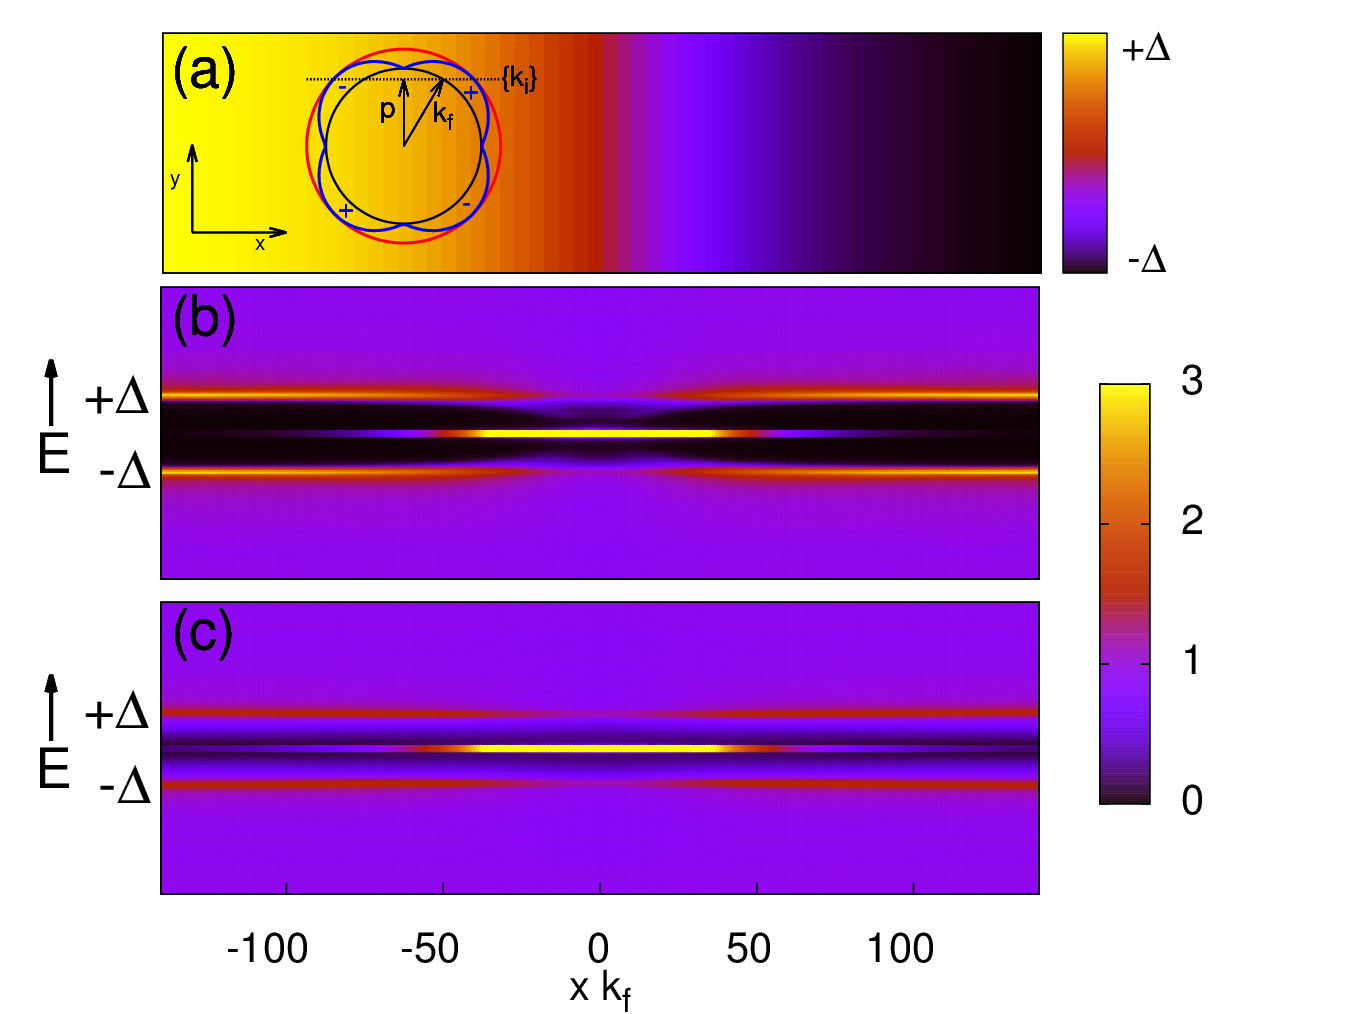
\includegraphics[scale=0.21]{./figures/fig1/Fig1.png}
\caption{\label{fig:1}
(a) Domain wall $+\Delta \to -\Delta$ in $x$-direction with translational
invariance along $y$. Inset shows orientation of the domain wall relative 
to internal symmetry of the order parameter, $S$ (red) or $D$-wave (blue), 
on the Fermi surface (black) in reciprocal space. 
%For each $p\hy$ we use the set of points $\{k_i\}\hat{x}$ to do a Fourier Transform.
%{\bf 1a right inset}: The applied Zeeman field H and deviation $\delta H$. 
(b) The normalized local density of states $N(\epsilon,x)/N_f$ for S-wave domain wall, and  
(c) the same for D wave. The zero-energy states appear at the domain wall. 
%All plots are against dimensionless length $xk_f$ for the horizontal coordinates. 
We use $\Delta_0=0.05\epsilon_f$ throughout the paper.  
%Parameters are: $\Delta_0=0.05\epsilon_f$, $k_BT=\mu_B H=0.05\Delta_0$, $\omega'' = \Delta_0/100$.  
\red{remove H-field arrows and label panels just (a)(b)(c), indicate 1 on cscale for DOS}
\blue{new figure is attached to email}
} 
\end{figure}
%%%%%%%%%%%%%%%%%%%%%%%%%%%%%%%%%%%%%%%%%%%%%%%%%%%%%%%%%%%%%%%%%%%%%%%%%%%%%%%%%

%~~~~~~~~~~~~~~~~~~~~~~~~~~~~~~~~~~~~~
\section{Model}
\label{sec:model}
%~~~~~~~~~~~~~~~~~~~~~~~~~~~~~~~~~~~~~
%
We work with the Hartree-Fock-Bogoliubov (HFB) mean-field Hamiltonian for a single band
\be
\label{eq:modelH} 
\cH_{HFB} = \frac{1}{2} \int d\vx d\vx'\quad{\Psi}^\dagger(\vx)\,{\cH}(\vx,\vx')\,{\Psi}(\vx') %+ const
\ee
where we have defined the field operator 
${\Psi}^\dag(\vx) = \left( \psi^\dag_{\uparrow}(\vx), \psi^\dag_{\downarrow}(\vx), 
\psi_{\uparrow}(\vx), \psi_{\downarrow}(\vx) \right)$, 
and ${\bf\cH}(\vx,\vx')$ is a $4\times 4$ block matrix
\be
 {\bf\cH}(\vx,\vx') = \left( \begin{array}{cc}
\hat{\cH}_{0}\,\delta(\vx-\vx') & \hat{\Delta}(\vx,\vx') \\
-\hat{\Delta}^*(\vx,\vx') & -\hat{\cH}_{0}^*\, \delta(\vx-\vx') 
\end{array} \right) \,.
\label{eq:modelHd}
\ee
$\hat{\cH}_{0}=\left[\frac{-\nabla^2}{2m^*} - \epsilon_f \right]\hat{1} - \mu_B H\sigma^z$ 
describes free electrons in a Zeeman field, 
$m^*$ is the effective mass of the electron, $\epsilon_f$ is the Fermi energy, 
$H$ is the applied magnetic field and $\mu_B$ is the Bohr magneton. 
%$\cI$ is the $2\times 2$ identity matrix, and 
$\sigma^{\alpha= \{x,y,z\}}$ are the Pauli matrices. 
The singlet superconducting pair potential is self-consistently defined as 
\bea
\hat{\Delta}(\vx,\vx') &=& (i\sigma^y)\Delta(\vx,\vx') \\
\label{eq:delta}
\Delta(\vx,\vx') &=& V(\vx-\vx')\langle \psi_{\beta}(\vx') \psi_{\alpha}(\vx) \rangle (i \sigma^y)_{\alpha\beta}
\eea
%appears in the off diagonals of ${\bf\cH}$, 
where summation over repeated spin indices is implied, and $\langle ... \rangle$ denotes ensemble average. 
$V(\vx-\vx')$ is the effective attractive interaction %between the electrons which 
that leads to superconductivity, with the cut-off energy $\Lambda$.
%and only affects electrons which are below the energy cut-off $\Lambda$.

Since we expect presense of degenerate zero-energy states we need to define 
Bogoliubov-Valatin canonical transformation with some care.\cite{MEschrig2015}
We take 
\bea
\label{eq:BdG_trans}
\left[\begin{array}{c} \psi_{\mu} \\  \psi^\dag_{\mu} \end{array} \right](\vx)
= \sum_{\vn}%{}^{'} %\left[ 
U^{(+)}_{\vn,\mu\nu}(\vx) \, \gamma_{\vn\nu} + 
U^{(-)}_{\vn,\mu\nu}(\vx) \, \gamma^\dag_{\vn\nu} 
\,, %\right] \,,
%\nonumber
\eea
where for inhomogeneous superconductor the state index $\vn$ replaces momenum $\vk$, 
used to label states in uniform superconductor. 
To treat the zero-energy states similarly to the other states, 
$\vn$ labels all positive energy states, and \emph{half} of zero-energy states, 
as we explain below. 
The $U^{(\pm)}_{\vn}(\vx)$ are two eigenvectors of the Hamiltonian (\ref{eq:modelHd}) 
corresponding to positive and negative energy branches 
\be
\int d\vx' \cH(\vx,\vx') U^{(\pm)}_{\vn}(\vx') = \pm \epsilon_\vn U^{(\pm)}_{\vn}(\vx)
\ee
Due to particle-hole symmetry of HFB Hamiltonian, for each $\vn$ there is a pair of $\pm\epsilon_\vn$ states, 
related to each other through
\bea
U^{(+)}_{\vn,\mu\nu}(\vx) = 
\left[\begin{array}{r} \delta_{\mu\nu} \, u_\vn \\  - i\sigma^y_{\mu\nu}v_{\vn} \end{array} \right] 
\quad,\quad
%\nonumber
%\\
U^{(-)}_{\vn,\mu\nu}(\vx) = 
\left[\begin{array}{r}  - i\sigma^y_{\mu\nu}v^*_{\vn} \\ \delta_{\mu\nu} \, u^*_\vn \end{array} \right] 
\nonumber
\eea
The non-zero energy states are naturally represented by $\gamma_{\vn \mu}$ and $\gamma^\dag_{\vn \mu}$ 
terms in (\ref{eq:BdG_trans}). However as a consequence of the particle-hole, 
the zero-energy states also come in pairs, and assignment of $\gamma_{0 \mu}$ or $\gamma^\dag_{0 \mu}$ 
to them is somewhat arbitrary. 
To avoid double-counting of zero-energy states in (\ref{eq:BdG_trans}), we take half of them and assign it to 
`positive' solutions ($\gamma$, $U^{(+)}$) and the other half appear as 
`negative' part ($\gamma^\dag$, $U^{(-)}$). 
%In this way the all the states are equivalent in the transformation...
To find the positive energy states we solve 
Bogoliubov-de Gennes equations, and in case of singlet superconductivity 
they are spin-independent: 
\begin{align}
\begin{split}
& \epsilon_{\vn}u_{\vn}(\vx)= \xi(-i\grad) u_{\vn}(\vx)+\int d\vx'\Delta(\vx,\vx')v_{\vn}(\vx') \\
& \epsilon_{\vn}v_{\vn}(\vx)= -\xi(-i\grad)^* v_{\vn}(\vx)+\int d\vx'\Delta^*(\vx,\vx')u_{\vn}(\vx')
\end{split}
\label{eq:BdG}
\end{align}
where $\xi(-i\grad) =  (-i\grad)^2/ 2m^* - \epsilon_f$. 
In Zeeman field The quasi-particle excitation energy is simply shifted from $\epsilon_\vn$ value by 
%and the energy of a quasi-particle excitation $\gamma^\dagger_{\vn\mu}$ is 
$\epsilon_{\vn\mu} = \epsilon_{\vn} - \mu_B H \, \sigma^z_{\mu\mu}$
and the Hamiltonaian in diagonal form is 
$\cH_{HFB} = E_0 + \sum_\vn \; %\limits_\vn \; %_{\vn;\,\mu=\uparrow,\downarrow} \; 
\epsilon_{\vn \mu} {\gamma}_{\vn \mu}^\dag {\gamma}_{\vn\mu}$. 
%($\hat{\epsilon}_{\vn} = diag[\epsilon_{\vn\uparrow},\epsilon_{\vn\downarrow},
%-\epsilon_{\vn\uparrow},-\epsilon_{\vn\downarrow}]$)
%${\bf\gamma}_{\vn}^\dag = (\gamma^\dag_{\vn\uparrow}, \gamma^\dag_{\vn\downarrow}, 
%\gamma_{\vn\uparrow}, \gamma_{\vn\downarrow})$ 
Finally, orthogonality of solutions with different $\vn$s, and orthogonality of 
positive and negative solutions result in two normalization conditions: 
\bea
\int d\vx\, \left[ u_{\vn}(\vx)u_{\vn'}^*(\vx) + v_{\vn}(\vx)v_{\vn'}^*(\vx) \right] &=& \delta_{\vn\vn'} \\
\int d\vx\, \left[u_{\vn}(\vx)v_{\vn'}(\vx) - v_{\vn}(\vx)u_{\vn'}(\vx) \right] &=& 0
\eea

For the domain wall or stripes configuration one has translational invariance along the wall ($\hy$) 
with momentum quantum numbers $\{p\}$, 
and in the transverse direction the wave function for given $p$ is expanded into Fourier Series
\be
\label{eq:wave_exp}
\begin{split}
u_{\vn}(\vx) = e^{ipy}\sum\limits_{j=0}^{N-1} \tilde{u}_{\vn}(k_j) e^{ik_jx}  \,,
\\
v_{\vn}(\vx) = e^{ipy}\sum\limits_{j=0}^{N-1} \tilde{v}_{\vn}(k_j) e^{ik_jx} \,.
\end{split}
\ee
We employ a Fast Fourier Transform technique with 
\[  \frac{k_j}{k_f} = \left\{
\begin{array}{ll}
       4\pi j/N, & j\leq N/2 \\
      -4\pi (N-j)/N, & j>N/2
\end{array} 
\right. \]
and periodic boundary conditions at $k_f x=0$ and $k_f x=N/2$ ($k_f$ is the
Fermi momentum). The reasons for beginning with a doubled Fourier domain
$(-2\pi,2\pi]$ is because the calculation of the relative momentum spin
susceptibility will half the domain to $(-\pi,\pi]$ while doubling the spatial
domain to $(-N/2,N/2)$. We use $N=2^{10}=1024$ \blue{The new plots are with $2^{12}=4096$ momentum grid points.}

For efficient numerics, we restrict our set of transverse momenta $\{k_j\}$ for each $p$ to include only those whose normal excitation energy 
\be
\xi(p,k_j) = \frac{k_j^2 + p^2}{2m^*} - \epsilon_f,
\ee
is below an energy cut-off, $|\xi_{p,k_j}|\leq\Lambda$. 
All higher energy solutions to (\ref{eq:BdG}) are considered normal with $\Delta(\vx,\vx') = 0$.

Furthermore, since we are interested in low-energy superconducting quasiparticles, 
we take a separable form of the pair potential, 
described by the amplitude that depends on the center of mass coordinate $\vR = (\vx + \vx')/2$, 
and the internal symmetry profile $g(\vr)$ that depends on the relative coordinate $\vr = \vx-\vx'$, 
\be
\Delta(\vR,\vr) = \Delta(\vR) \, \left[ \int \frac{d\vL}{(2\pi)^2}\,  g_{\hat{L}} e^{i\vL\cdot\vr} \right] \,,
\ee
where $\vL$ is the relative momentum in a Cooper pair. 
We will consider pairing states $l=0$ (S wave) and $l=2$ (D wave)
\be
\label{eq:rot_sym}
\begin{split}
S-wave:\quad& g_{\hat{L}} = 1 \\
D-wave:\quad& g_{\hat{L}} = \sin(2\theta_{\hat{L}})
\end{split}
\ee
$\theta_{\hat{L}}$ is the angle of $\vL$ measured from the x-axis. 
The profile of the order parameter across the domain wall depends only on coordinate $x$, $\Delta(\vR) = \Delta(x)$.
%and we further specify the profile
%$\Delta(\vR)\!\!\!\Rightarrow\!\!\!\Delta(R)$ only depends on the $\hx$ CoM
%($R=\vR\cdot\hx$) for striped geometry.

Using equations (\ref{eq:wave_exp}) for the amplitudes, (\ref{eq:BdG}) becomes
a matrix eigenvalue equation for $\epsilon_{\vn}$, where the $2N$ Fourier
coefficients, $\tilde{\cU}_{\vn}^T =
(\tilde{u}_{\vn}(k_0),\,\tilde{u}_{\vn}(k_1) ...\tilde{u}_{\vn}(k_{N-1}),
\tilde{v}_{\vn}(k_0),\,\tilde{v}_{\vn}(k_1)...\tilde{v}_{\vn}(k_{N-1}))$ 
form the eigenvector for each longitudinal momentum $p$, 
\be
\label{eq:BdG_mat}
\epsilon_{\vn}\tilde{\cU}_{\vn}
=\left( \begin{array}{cc}
\vvec{\xi}_{p} & \vvec{\Delta}_{p} \\
\vvec{\Delta}^*_{p} & -\vvec{\xi}_{p}  \end{array} \right)
 \tilde{\cU}_{\vn}
\ee
where $\vvec{\xi}_{p}$ and $\vvec{\Delta}_{p}$ are $N\times N$ matrices with $(i,j)th$ entries
\bea
\label{eq:NxN}
\vvec{\xi}_{p}(i,j) = \left(\frac{k_i^2 + p^2}{2m_e} - \epsilon_f \right)\delta_{ij} \\
\vvec{\Delta}_{p}(i,j) =  g_{\hat{L}_{ij}} \int dx\, \Delta(x) e^{-i(k_i-k_j)x}
\eea
where $\vL_{ij} = \frac{k_i+k_j}{2} \hx + p\hy$. 
Solving (\ref{eq:BdG_mat}) we obtain $2N$ eigenstates, out of which $N$ have positive (and zero) energies, 
and $N$ has mirror negative (and zero) energies. 
We arrange solutions from negative to positive 
energies, and the quantum number $\vn = (p,n)$ labels top $N$ energy states. 
This guarantees that it goes over all positive $\epsilon_\vn$ and half of zero-energy solutions. 

We consider a system where we apply a unifrom static field $\vH_0$, and consider a magnetic 
response to a small perturbation of the magnetic field 
$\delta \vH(\vx,\omega) = \int dt e^{i\omega t} \delta \vH(\vx,t)\Theta(t)$, 
where $\Theta(t)$ is the Heaviside step function. Up to first order in perturbation the electron magnetization is
\bea
\label{eq:delM}
%\vM_\alpha(\vx,\omega) = \langle \vS_\alpha(\vx,\omega)\rangle + \delta\vM_\alpha(\vx,\omega) \\
M_\alpha(\vx,\omega) = M_{0,\alpha} + \delta M_\alpha(\vx,\omega) \\
\delta M_\alpha(\vx,\omega) = \int d\vx' \; \chi_{_{\alpha\beta}}(\vx,\vx',\omega) \, \delta H_{\beta}(\vx',\omega)
\eea
where $\vM_0$ is the magnetization in the superconducting state due to the uniform field $\vH_0$. 
The bare susceptibility $\chi_{_{\alpha\beta}}(\vx,\vx',\omega)$ is 
given by the Kubo formula\cite{doi:10.1143/JPSJ.12.570}
\be 
\label{eq:sus_def}
\chi_{_{\alpha\beta}}(\vx,\vx',\omega) = i\mu_B^2\int dt \; e^{i\omega t} \, 
\langle [S_\alpha(\vx,t), S_\beta(\vx',0)]\Theta(t) \rangle 
\ee
where 
$\vS(\vx,t) = \sum_{\mu\nu} \psi_\mu^\dagger(\vx,t) \vsigma_{\mu\nu}
\psi_\nu(\vx,t)$ is the spin operator and $\omega = \omega' + i\omega''$ is
assumed to have a small imaginary part ($\omega''\ll \Delta_0$, the gap energy $T=0,H=0$) 
for convergence of the time integration. 

Without effects that introduce spin-orbit coupling, the isotropy of spin space is 
broken only by $\vH_0$. 
Then the susceptibility tensor is diagonal in 
longitudinal($\delta\vH \parallel \vH_0$)-transverse($\delta\vH \perp \vH_0$) space. 
We are mostly interested cases when the induced or spontaneous magnetization is orthogonal to 
uniform state $\delta\vM(\vq,\omega) \perp \vM_0$.
Using the Bogoliubov-Valatin transformation, the \red{normalized ?} \blue{yes, it is normalized to $\chi_0$} transverse susceptibility is 
\be
\begin{split}
\label{eq:sus}
\chi_{_{\perp}}(\vx,\vx',\omega) = \frac{2\mu_B^2}{\chi_{_0}} \sum\limits_{\vn\vn'\mu} 
  & \left[ A_{\vn\vn'}(\vx)A^*_{\vn\vn'}(\vx') \Pi_{\vn\mu;\vn'\bmu}^{+}(\omega) \right.  \\
+ &\frac{1}{2}C^*_{\vn\vn'}(\vx)C_{\vn\vn'}(\vx') \Pi_{\vn\mu;\vn'\mu}^{-}(\omega) \\ 	
+ & \left. \frac{1}{2}C_{\vn\vn'}(\vx)C^*_{\vn\vn'}(\vx') \Pi_{\vn\mu;\vn'\mu}^{-}(-\omega) \right] 
\end{split}
\ee
Here $\bmu$ denotes spin state opposite to $\mu$, 
\be
\label{eq:fermi_factor}
\Pi_{\vn\mu;\vn'\nu}^{\pm}(\omega) = \frac{f(\epsilon_{\vn \mu}) - f(\pm\epsilon_{\vn' \nu})}
{\omega+\epsilon_{\vn \mu} \mp \epsilon_{\vn' \nu}} \,,
\ee
$f(\epsilon)$ is the Fermi distribution function, 
and $\chi_{_0}=2\mu_B^2N_f$ is the Pauli susceptibility with normal state density of state 
at the Fermi energy per spin projection $N_f$. 
For energies close to zero, or much less than temperature spread of the Fermi-Dirac distribution, 
\be
\Pi_{\vn\mu;\vn'\nu}^{\pm}(\omega) \approx \pder{f}{\epsilon} 
\frac{\epsilon_{\vn \mu} \mp \epsilon_{\vn' \nu}}
{\omega+\epsilon_{\vn \mu} \mp \epsilon_{\vn' \nu}} 
%= \frac{1}{4T} \frac{\epsilon_{\vn \mu} \mp \epsilon_{\vn' \nu}}
= \frac{\epsilon_{\vn \mu} \mp \epsilon_{\vn' \nu}}
{4T(\omega+\epsilon_{\vn \mu} \mp \epsilon_{\vn' \nu})}  
\,.
\nonumber
\ee
Combinations of quasiparticle amplitudes 
\bea
A_{\vn\vn'}(\vx) = u^*_{\vn}(\vx)u_{\vn'}(\vx)+v^*_{\vn}(\vx)v_{\vn'}(\vx) \\
C_{\vn\vn'}(\vx) = u_{\vn}(\vx)v_{\vn'}(\vx) - v_{\vn}(\vx)u_{\vn'}(\vx)
\eea
give the `coherence factors'. They determine the spatial dependence of
susceptibility, while the remaining terms are functions of the energy and
temperature. 

We note that the combinations $A_{\vn\vn'}(\vx)A^*_{\vn\vn'}(\vx')$ and
$C^*_{\vn\vn'}(\vx)C_{\vn\vn'}(\vx')$ in (\ref{eq:sus}) 
under coordinate exchange 
$\vx\leftrightarrow\vx'$ ($\vr\leftrightarrow -\vr$) become complex conjugated. 
This symmetry guarantees that local susceptibility at wave vector $\vq$ 
\be
\label{eq:sus_trans}
\chi_{}(\vq,\vR,\omega) = \int d\vr \; e^{-i\vq\cdot\vr} \chi_{}(\vr,\vR,\omega),
\ee
has real part $\chi'$ that depends only on the \emph{real} part of $\Pi_{\vn\mu;\vn'\nu}^{\pm}$, 
and the imaginary part $\chi''$ has contributions only from the \emph{imaginary} part of $\Pi_{\vn\mu;\vn'\nu}^{\pm}$. 
%for a particular term $(\vn\mu;\vn'\nu)$, the contribution to 

Lastly, we find the spin-lattice relaxation rate $T_1^{-1}$ due to the
hyperfine interaction between nuclear spins $\vI(\vx_s)$ and electron spins
$\vS(\vx)$
\be
\cH_{hf} = \int d\vx d\vx_s \, \vI(\vx_s) \cdot { \cA}(\vx_s-\vx) \cdot \vS(\vx)
\ee
${ \cA}(\vr)$ is the $3\times 3$ hyperfine matrix. For transitions
between spin 1/2 nuclear states which are well below the thermal energy
($\epsilon_i-\epsilon_f=\omega<<T$), and if ${ \cA}(\vr)$ is strongly peaked near 
$\vr=0$, the spin-lattice relaxation rate due to ${\cA}_{\perp}$ is
found using first order perturbation theory, \cite{nmr_abragam}
\be
\label{eq:rel_time}
T_1^{-1}(\vR,\omega) = 2T\lim\limits_{\omega\rightarrow 0}\sum\limits_{\vq}
\quad |\cA_{\perp}(\vq)|^2 \frac{\chi''_{_{\perp}}(\vR,\vq,\omega)}{\omega}
\ee
The details of $\cA_{\perp}(\vq)$ depend on the interactions of the spin
fields, however in an effort to focus on the DW effects we consider only the
simplest isotropic coupling, $\cA_{\perp}(\vq) = A_0$. 

%~~~~~~~~~~~~~~~~~~~~~~~~~~~~~~~~~~~~~
\section{Results and Analysis}
\label{sec:AandR}
%~~~~~~~~~~~~~~~~~~~~~~~~~~~~~~~~~~~~~
We first find the profile of the order parameter for the 
domain wall configuration. The details of the self-consistently calculation are 
presented in appendix \ref{app:self-cons} and the general solution is shown in Fig.~\ref{fig:1}(a). 
The local density of states for spin projection $\mu$ is 
$ N_\mu(\epsilon,\vx) = -(1/\pi) \Im[G^R_{\mu}(\epsilon,\vx)]$ where $G^R_{\mu}(\epsilon,\vx)$ 
is the retarded Greens function, 
\begin{align} 
\begin{split}
G^R_\mu(\epsilon,\vx) = -i \int\limits_0^\infty dt\; e^{i(\epsilon+i0) t} 
\langle [\psi_{\mu}(\vx,t) \,,\, \psi_{\mu}^\dagger(\vx,0) ]_+ \rangle \\ %\Theta(t) \\ 
= \sum_{\vn}\left[ 
\frac{|u_{\vn}(\vx)|^2}{\epsilon - \epsilon_{\vn\mu} + i0} 
+ \frac{|v_{\vn}(\vx)|^2}{\epsilon + \epsilon_{\vn\bmu} +i0}\right] 
\end{split} 
%\label{eq:ldos} 
\nonumber
\end{align}
average $\langle\dots\rangle$ is over the ground state of the superconductor.  
LDOS is presented in figure \ref{fig:1}(b,c) for S- and D-wave pairings. The large zero-energy peak 
appears at the domain wall, confined on the scale of $10\xi_c$ ($\xi_c = v_f/2\pi T_c$).
In magnetic field the spectrum is Zeeman-shifted and the bound states appear at energies $\pm \mu_B H_0$ for up/down
spins. 
We perform calculations by introducing a cutoff in energy $\Lambda = 5 \Delta_0$, above which we treat states 
as if in normal metal. We set zero-temperature gap in terms of Fermi energy $\Delta_0 = 0.05\epsilon_f$, which results in coherence 
lengths $\xi_{c}^s = 11.2/k_f$ (S-wave) and  $\xi_{c}^d = 13.6/k_f$ (D-wave). 
The cutoff provides a rough separation of low and high energy scales, and one can break the double 
sum over $\vn$ and $\vn'$ in susceptibility (\ref{eq:sus}) into three contributions
\be
\begin{array}{c@{\qquad}l@{\qquad}l}
I & \epsilon_{\vn} <\Lambda, \; \epsilon_{\vn'}<\Lambda & \mbox{low-$\epsilon$}
\\
II  & \epsilon_{\vn} <\Lambda, \; \epsilon_{\vn'}>\Lambda; \quad (\vn\leftrightarrow \vn') & \mbox{mixed-$\epsilon$}
\\
III & \epsilon_{\vn} >\Lambda, \; \epsilon_{\vn'}>\Lambda   & \mbox{high-$\epsilon$}
\end{array}
\nonumber
\ee

%%%%%%%%%%%%%%%%%%%%%%%%%%%%%%%%%%%%%%%%%%%%%%%%%%%%%%%%%%%%%%%%%%%%%%%%%%%%%%%%%
\begin{figure*}
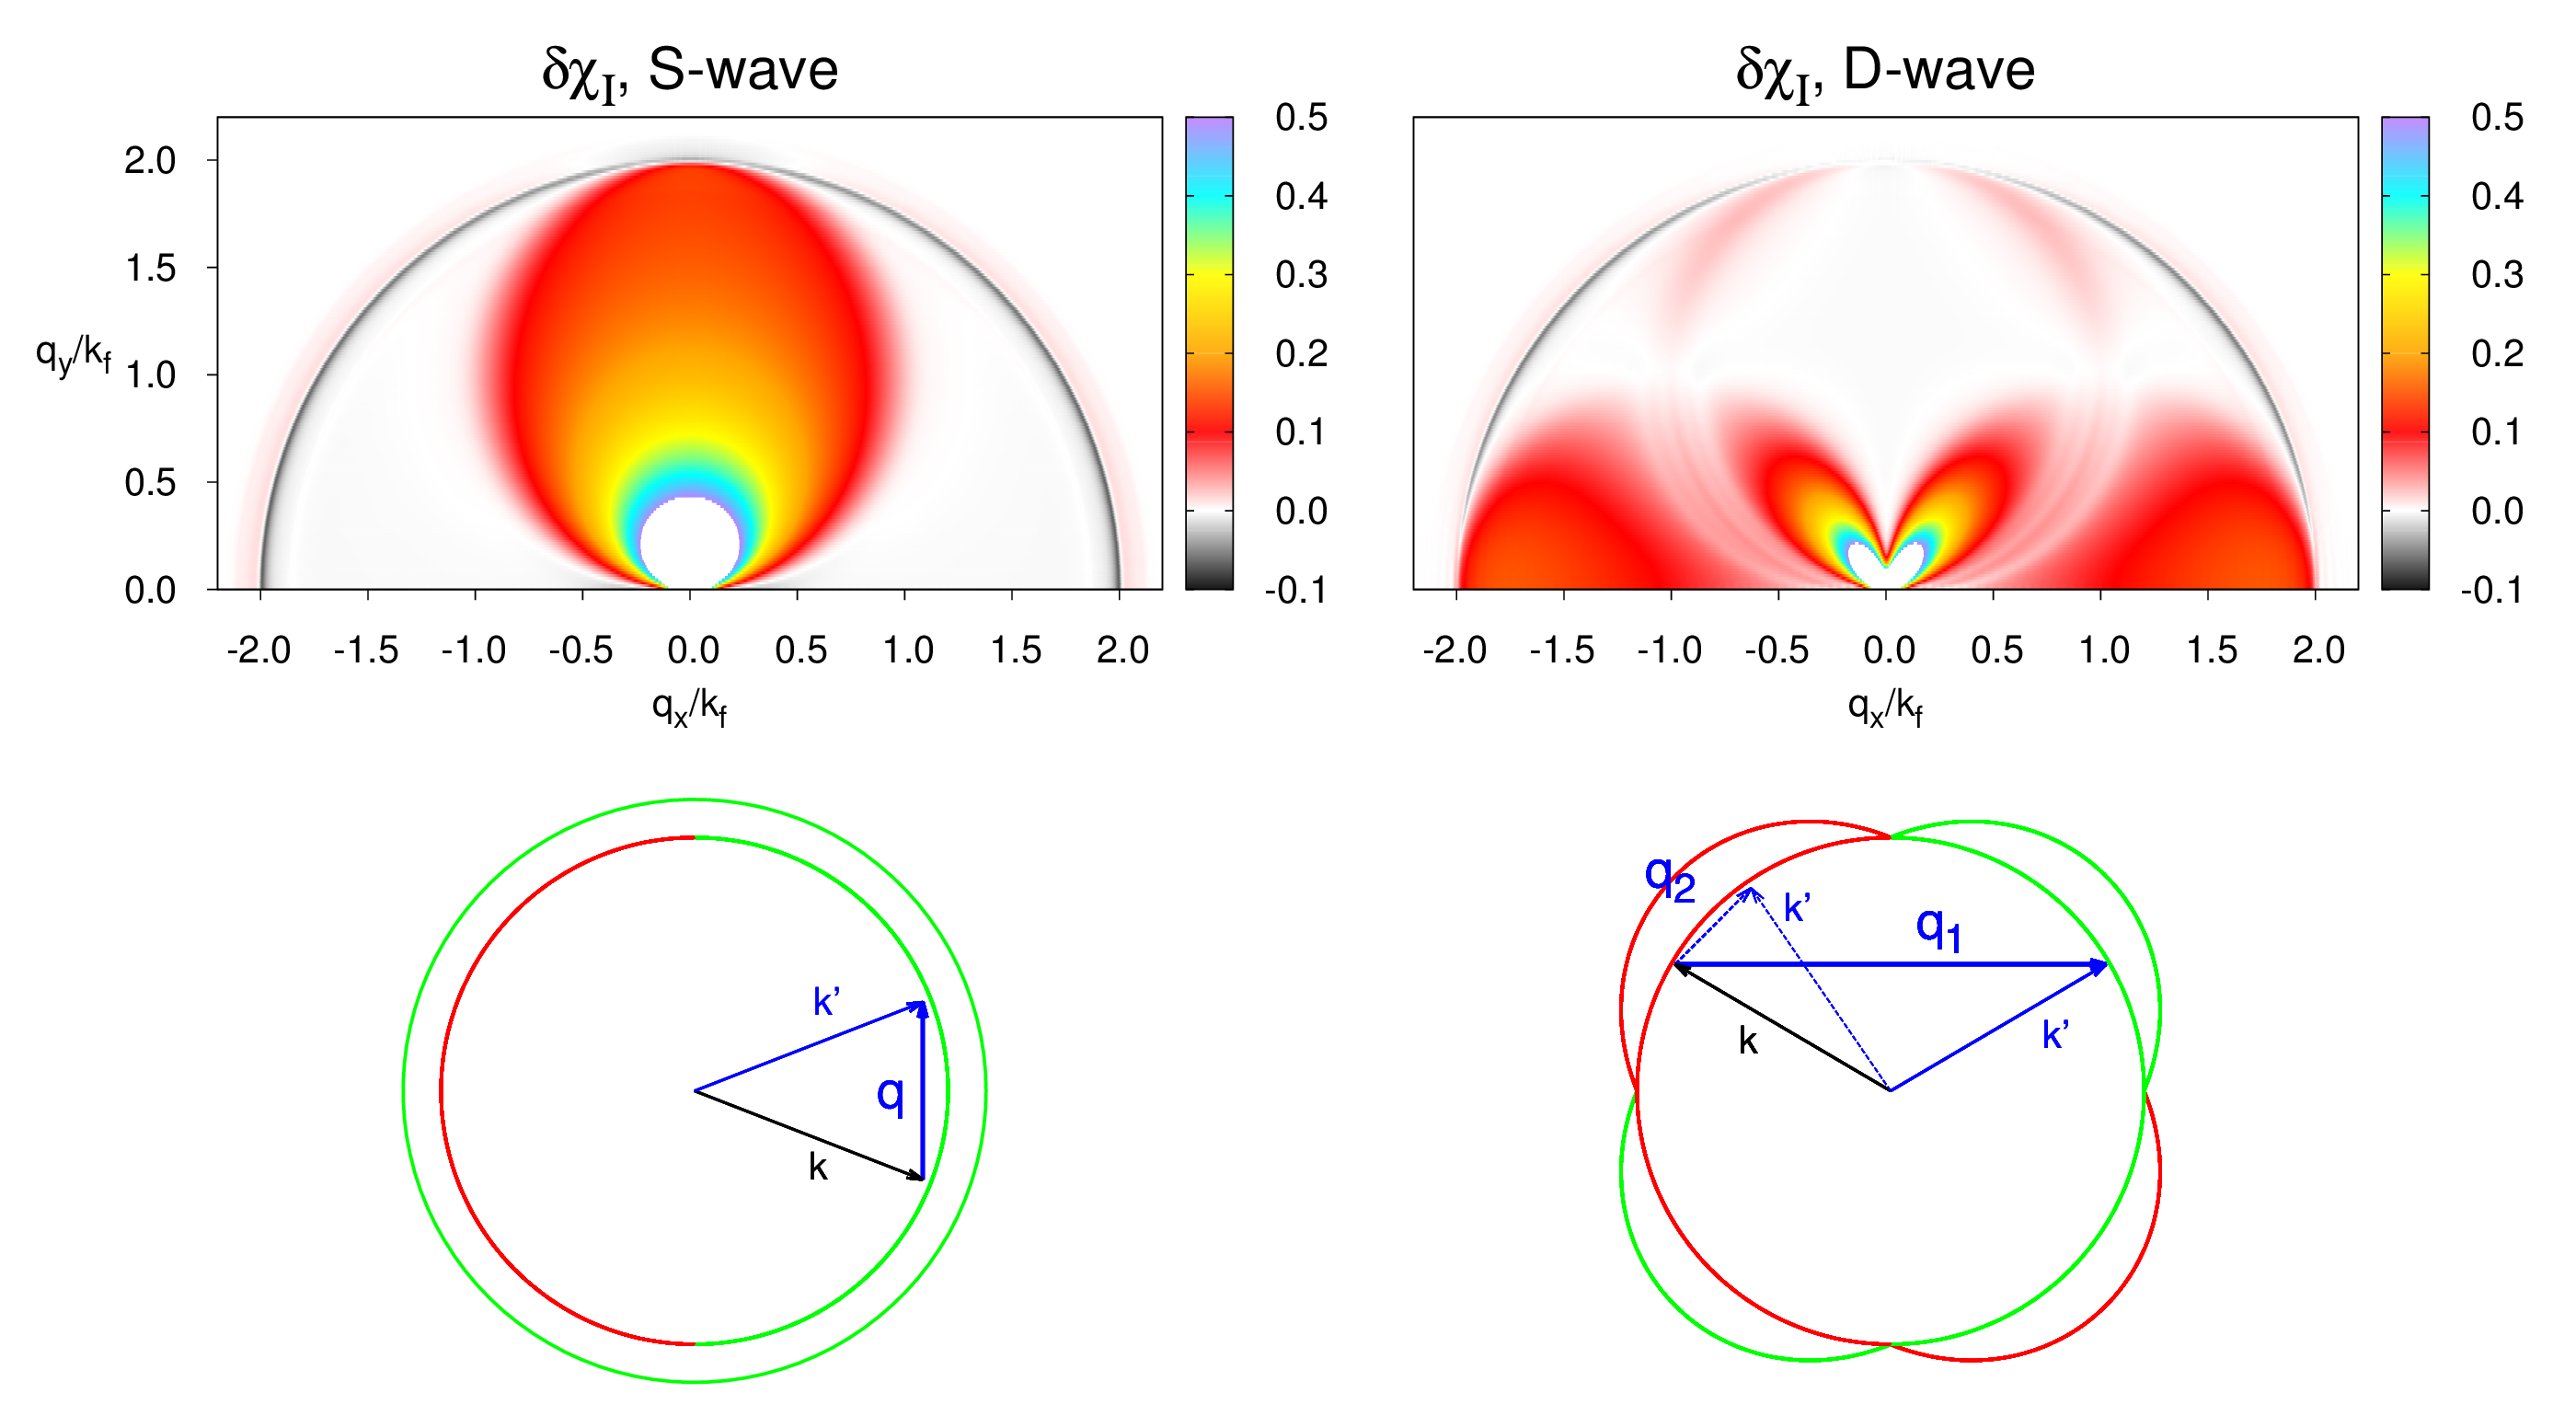
\includegraphics[scale=0.17]{./figures/fig2_SD_andreev/Fig2_andreev.png}
\caption{\label{fig:2}
Upper panels show zero-field low-temperature susceptibility $\delta\chi'(\vq,0,0)$ 
as a function of ordering vector $\vq$,  at the center of the domain wall. 
%at $\mu_B H=0.01\Delta_0$ and $k_BT = 0.01\Delta_0$. 
The white region around $\vq=0$ (uniform magnetization) has enhancement $\delta\chi'>0.5$ due to large density of 
bound states and has been removed to better highlight the main features. 
The $S$-wave superconductor favors $\vq || \hy$ along the domain wall. A domain wall in $D$-wave 
increases tendency for AFM with $q_x \sim 1.75 k_f$ across the domain wall. 
%
Bottom panels shows ordering vectors $\vq$ that connect points on the Fermi surface with same signs of 
$\Delta_{\hk f }$ and $\Delta_{\hk' f }$ that give largest coherence factors between zero-energy bound states. 
The OP at the final end of quasiclassical trajectory $\hk$, $\Delta_{\hk f }$, 
is a product of the domain wall spatial profile (inner circle) 
and the symmetry $g_{\hk}$ (outer profile). Red/green denote signs $\mp1$. 
%
\red{switch top and bottom rows; plot $\delta \chi$, not $\delta\chi_I$; 
smaller FS schematics and remove red arrows, GREEN and RED are bad together; 
DO NOT USE red or any other colors that resemble 
color palette for contours. 
use GREEN maybe and 3 different line styles. Or maybe just show contours without the colors - good for B/W? 
SAME FOR NEXT FIGURE.}
\blue{new figure attached. I really cant plot full $\delta \chi$, at least not with nearly as high accuracy as $\delta \chi_I$. My plan was to focus on low-$\epsilon$ only. Note, these are not exactly zero field, I used $\mu_B H/\Delta_0=0.01$ and $k_B T/\Delta_0=0.05$}
} 
\end{figure*}
%%%%%%%%%%%%%%%%%%%%%%%%%%%%%%%%%%%%%%%%%%%%%%%%%%%%%%%%%%%%%%%%%%%%%%%%%%%%%%%%%

%~~~~~~~~~~~~~~~~~~~~~~~~~~~~~~~~~~~~~
\subsection{Real Susceptibility}
\label{sec:realChi}
%~~~~~~~~~~~~~~~~~~~~~~~~~~~~~~~~~~~~~
We calculate the deviation of local susceptibility in non-uniform superconductor from the known normal state value 
\be
\delta\chi(\vq,x,\omega) = \chi(\vq,x,\omega) - \chi^{N}(|\vq|,\omega) \,,
\ee
which means cancellation of high-energy part $III$ in (\ref{eq:sus}). 
Mixed terms $II$ are affected by superconductivity and the domain wall, but we
find the deviations of these terms from their normal state values to be small 
compared to changes in low-energy terms $I$, which strongly dominate $\delta\chi$. %experience the most dramatic effects.
%\be \delta\chi_{_I}(\vq,R,\omega) = \chi_{_I}(\vq,R,\omega) - \chi_{_I}^{N}(\vq,\omega) \ee
%

In figure \ref{fig:2} we show zero-field results for local static susceptibility ($\omega=0$) in the middle of the domain wall ($x=0$) 
as a function of the ordering vector $\vq$. 
\red{We find that the full deviation from the normal state value $\delta\chi(\vq,0,0)$ on 
99.9\% is given by the low-energy contribution $\delta\chi_I$ - PUT NUMERICAL EVALUATION OF THE DIFFERENCE $II$}. \blue{$|\delta\chi_{II}|<\Delta/\epsilon_f$ everywhere and much less for most $\vq$. Should we move this to the previous paragraph? I haven't thought about $II$ for awhile so I don't have any recent data to plot. I thought region $II$ was outside the scope of this paper.}
The susceptibility is clearly increased for uniform magnetization $q\approx0$, due to large density of bound states at 
zero energy. There are also several regions of non-zero $q \sim k_f$, for which $\chi_\perp$ is significantly enhanced over the normal
state value, showing tendency towards antiferromagnetic ordering. 
In $S$-wave superconductor, Fig.~\ref{fig:2}(left), the direction of such $\vq$ vectors is along the $y$-axis, i.e. pointing along the domain
wall. We find that similar results happen for $D_{x^2-y^2}$-wave, when the domain wall is along the maximum gap
directions. 
%
When the domain wall is along nodes of $D$-wave order parameter, Fig.~\ref{fig:2}(right), the ordering vector $\vq$ showing enhanced 
susceptibility is along the diagonal directions for small $q_y/k_f \approx \pm q_y/k_f$, 
and for $q_x \sim 1.75 k_f$ that shows about 15\% enhancement over $\chi_0$. 
The latter means that if antiferromagnetic SDW order is induced by the non-uniform superconductivity, 
its modulation vector will be normal to the order parameter domain wall, or normal to the 
pairbreaking surface if we consider semi-infinite superconductor. %or $\vq_{AFM} || \vq_{FFLO}$. 

We associate these regions of enhancement exclusively with correlations between bound states. 
Overall, one expect biggest change in the static $\omega=0$ susceptibility from terms in 
(\ref{eq:sus}) that have vanishing denominators of (\ref{eq:fermi_factor}) i.e.  
$\epsilon_{\vn\mu}\pm\epsilon_{\vn'\mu'} \to 0 $. 
Thus, the $(\vn\mu;\vn'\nu)$ term
which connects two bound states with zero energies should give a large contribution. 
The magnitude of this contribution, however, is also determined by the phase space, 
or the weight of zero-energy state,
and spatial dependence of the coherence factors. 

To understand the role of coherence factors one can use Andreev approximation to estimate the BdG
$u_\vn,v_\vn$ amplitudes. 
The state index can be written as $\vn=(\hk,n)$, where $\hk$ is the unit vector that defines a quasiclassical
trajectory, and $n$ labels states along this trajectory:
$$
u_\vn(\vx) = u_{\hk,n}(\vx) e^{ip_f \hk \cdot \vx}  \,,
\qquad
v_\vn(\vx) = v_{\hk,n}(\vx) e^{ip_f \hk \cdot \vx}  \,.
$$
Then Andreev equations follow from BdG equations (\ref{eq:BdG}): 
\begin{align}
\begin{split}
& (\epsilon_{\hk,n} + iv_f \hk\grad) u_{\hk,n}(\vx) = \Delta(\vx,p_f\hk) v_{\hk,n}(\vx) 
\\
& (\epsilon_{\hk,n} - iv_f \hk\grad) v_{\hk,n}(\vx) = \Delta^*(\vx,p_f\hk) u_{\hk,n}(\vx) 
\end{split}
\label{eq:Andreev}
\end{align}
By approximating the domain wall profile with a step function 
$\Delta(x, p_f \hk) = \Delta \sign(x) \; g_{\hk}$
the amplitudes for the zero-energy bound states are, 
\be
\label{eq:uv_andreev}
\left[ \begin{array}{c}
u_{\hk,n} \\ v_{\hk,n}
\end{array} \right] (\vx)
= \frac{1}{\sqrt{2}} 
\left[ \begin{array}{c}
1  \\ -i \; \sign(\Delta^*_{\hk f}) 
\end{array} \right] 
\exp\left(- \left| \frac{\Delta g_{\hk} \,x}{ v_f \hk_x} \right| \right)
%\begin{split}
%u_{\vn}(\vx)\propto e^{ip_f \hk\cdot\vx-\kappa |\hk\cdot\vx|}e^{\frac{i}{2} [\theta_{\vn} + \phi_{\hk,\vx}]} \\
%v_{\vn}(\vx)\propto e^{ip_f \hk\cdot\vx-\kappa |\hk\cdot\vx|}e^{-\frac{i}{2} [\theta_{\vn} +\phi_{\hk,\vx}]}
%\end{split}
\ee
where $\Delta$ is the bulk amplitude of the order parameter, % in direction $\hk$, 
and $\Delta_{\hk f} = \Delta \sign(\hk_x) \, g_{\hk}$ 
is the order parameter at the \emph{final} end of the quasiclassical trajectory $\hk$. 
%$\epsilon_{\vn} = \sqrt{(v_f\kappa)^2+\Delta_{\hk}^2}$, $\theta_{\vn} =
%\sign(\hk\cdot\hx)\cos^{-1}(\epsilon_{\vn}/\Delta_{\hat{k}})$, and the energies $\epsilon_{\vn\mu} = \epsilon_{\vn} -
%\sigma^z_{\mu\mu}\mu_B H$. $\phi_{\hk,\vx}$ is the OP phase as a function of $\hat{k}$ and $\vx$.
Using this one finds that the coherence amplitudes
between bound states at points $\hk, \hk'$ on the Fermi surface 
in the middle of the domain wall ($\vx=-\vx'=\vr/2$) are 
\begin{align} 
\label{eq:AA_andreev}
\begin{split}
%A_{\vn\vn'}(\vx)A^*_{\vn\vn'}(\vx') \propto
%e^{-ip_f(\hk-\hk')\cdot\vr-2\kappa_{\vn} |\hk\cdot\vr|-2\kappa_{\vn'} |\hk'\cdot\vr|} *\cos^2(\zeta_{\vn\vn'}/2)
A^0_{\hk\hk'}(\vx) A^{0}_{\hk\hk'}(\vx')^* 
= \left|\frac{1 + \sign( \Delta_{\hk f } \Delta^*_{\hk' f } )}{2}\right|^2 \qquad 
\\
\times \; e^{-ip_f(\hk-\hk')\cdot\vr}  \; 
e^{- \frac{\Delta}{v_f} \left( \left| \frac{g_{\hk}}{\hk_x} \right| +  \left| \frac{g_{\hk'}}{\hk'_x} \right|\right) 
 | \vr\hx|}
\end{split}\end{align}
%
\begin{align} 
\label{eq:CC_andreev}
\begin{split}
C^0_{\hk\hk'}(\vx) C^{0}_{\hk\hk'}(\vx')^* 
= \left|\frac{1 - \sign( \Delta_{\hk f } \Delta^*_{\hk' f } )}{2}\right|^2 \qquad
\\
\times \; e^{ip_f(\hk+\hk')\cdot\vr}  \; 
e^{- \frac{\Delta}{v_f} \left( \left| \frac{g_{\hk}}{\hk_x} \right| +  \left| \frac{g_{\hk'}}{\hk'_x} \right|\right) 
 | \vr\hx|}
\end{split}\end{align}
%\be\begin{split}
%\label{eq:CC_andreev}
%C_{\vn\vn'}(\vx)C^*_{\vn\vn'}(\vx') \propto
%e^{-ip_f(\hk+\hk')\cdot\vr-2\kappa_{\vn} |\hk\cdot\vr|-2\kappa_{\vn'} |\hk'\cdot\vr|} \\ *\sin^2(\zeta_{\vn\vn'}/2)
%\end{split}
%\ee
%and $\zeta_{\vn\vn'} = \theta_{\vn}+\phi_{\hk}-\theta_{\vn'}-\phi_{\hk'}$. The
%$AA^*$ term reaches a maximum when $\zeta_{\vn\vn'} = 0$ or $2\pi$ while $CC^*$
%is maximum for $\zeta_{\vn\vn'} = \pm\pi$. Employing continuous boundary
%conditions at the DW results in the bound states having $\epsilon_{\vn} = 0$,
%$\theta_{\vn}=\sign(\hk\cdot\hx)\frac{\pi}{2}$ and we can write the $\hk$ phase
%as $\phi_{\hk} = \frac{\pi}{2}(\sign(\Delta_{\hk}) -1)$ so that
%\be
%\zeta_{\vn\vn'} = \frac{\pi}{2}[\sign(\hk\cdot\hx) +\sign(\Delta_{\hk})- \sign(\hk'\cdot\hx) - \sign(\Delta_{\hk'})]
%\ee
The ordering vector $\vq= p_f(\hk-\hk') $ that maximizes $AA^*$ in (\ref{eq:AA_andreev}) 
corresponds to combinations of $\hk$ and $\hk'$ that 
have same sign of $\Delta_{\hk f }$ and $\Delta_{\hk' f }$. 
For $CC^*$ the ordering vector is $\vq = p_f(\hk+\hk')$ and with replacement $\hk' \to -\hk'$ 
Eq.~(\ref{eq:CC_andreev}) results in the same relation between $\Delta_{\hk f }$ and $\Delta_{\hk' f }$. 
These vectors are illustrated in the bottom panel of figure \ref{fig:2}. 
For $S$-wave $g_{\hk}=1$, and the two trajectories must end up on the same side of the domain wall, 
resulting in the $\vq$ ordering along the domain wall. For $D$-wave, the two trajectories 
can be inside the same lobe on the same side of the domain wall giving small $q_2$ vectors, 
or there is a large wavevector $q_1 \sim 2 k_f$ \blue{Isnt this $q_1 \sim 1.75 k_f$?} that connects points on the opposite lobes with trajectories 
ending up on different sides of the domain wall. 


But, the other \red{WHICH OTHER - the invisible ones?! - example is needed} \blue{The thin regions near $2k_f$ appearing in $S$ and $D$-wave for low field from terms connecting bound states and low lying free states. Also, the blob near $q=(0.7\hx,1.5\hy)$ and the regions between and around the main two enhanced spots for $D$-wave which is from the near nodal quasiparticles pairing with bound states. your explanation in the next paragraph is good for these} regions that increase above the normal
value cannot be from bound state pairs because these wave vectors have zero
amplitude from equations (\ref{eq:AA_andreev}) and (\ref{eq:CC_andreev}). 

Another set of ordering vectors can be obtained if one considers correlations between 
the bound states and the propagating states with energies 
$\epsilon_{\vn} \gtrsim |\Delta_{\hk}|$, small for 
directions $\hk$ close to nodes of $D$-wave, or along the domain wall $\hk = \hy$ with 
suppressed order parameter amplitude. The small energies are favorable 
to minimize the denominator in equation
(\ref{eq:fermi_factor}). The free-propagating particle (p) and hole (h) type 
solutions $e^{\pm i k \hk\cdot \vx}$ are  
\be
\label{eq:uv_andreev_free}
\left[ \begin{array}{c}
u_{\hk,n} \\ v_{\hk,n}
\end{array} \right] %(\vx)
\propto %\frac{1}{\sqrt{2}} 
\left[ \begin{array}{c}
\epsilon + v_f k %\sqrt{\epsilon^2 - |\Delta_{\hk}|^2}   
\\ \Delta^*_{\hk} 
\end{array} \right]
e^{i k \hk\cdot \vx}
%e^{i \sqrt{\epsilon^2 - |\Delta_{\hk}|^2} \hk\cdot \vx/v_f}
\,,\,
\left[ \begin{array}{c}
\Delta_{\hk}  \\ \epsilon + v_f k %\sqrt{\epsilon^2 - |\Delta_{\hk}|^2}   
\end{array} \right]
e^{-i k \hk\cdot \vx}
%e^{-i \sqrt{\epsilon^2 - |\Delta_{\hk}|^2} \hk\cdot \vx/v_f}
\ee
with $ v_f k = \sqrt{\epsilon^2 - |\Delta_{\hk}|^2}$. 
% \be
% \label{eq:uv_andreev_free}
% \begin{split}
% u_{\vn}(\vx)\propto e^{i\vk\cdot\vx}e^{\frac{1}{2} [\pm\chi_{\vn} + i\phi_{\hk,\vx}]} \\
% v_{\vn}(\vx)\propto e^{i\vk\cdot\vx}e^{-\frac{1}{2} [\pm\chi_{\vn} + i\phi_{\hk,\vx}]}
% \end{split}
% \ee
Considering particle and hole scattering on the domain wall, we can find the exact wave functions of 
the propagating states along $\hk$. For energies near the continuum edge, the eigenvectors are 
$
\left[ \begin{array}{cc} u_{\hk,n} \,,& v_{\hk,n} \end{array} \right] 
\propto 
\left[ \begin{array}{cc} 1 \,,& \sign(\Delta_{\hk})  \end{array} \right]
$
times appropriate reflection/transmission coefficients. 
The main feature of the propagating solutions is that they are real. 
Then combination of a bound state vector (\ref{eq:uv_andreev}) for $\hk$ with 
propagating state vector for $\hk'$ results in 
\be
\label{eq:AA_bf}
A_{\hk\hk'} A_{\hk\hk'}^* \, (0,\vr) \propto 
e^{-ip_f(\hk-\hk')\cdot\vr}  \; 
e^{- \frac{\Delta}{v_f} \left( \left| \frac{g_{\hk}}{\hk_x} \right|\right) | \vr\hx|}
\ee
where dependence on signs of the order parameter has disappeared, 
and similar for $CC^*$. 
This means that the coherence factors for such correlations do not 
introduce any extra angular dependence for ordering vectors $\vq$ \blue{other than the angular distribution of the bound states and orientation of the nodal directions of the $D$-wave}.  
We note, however, that such correlations at the domain wall are weighted by the 
particle/hole transmission and reflection coefficients,  
that can be quite small for $\epsilon \gtrsim |\Delta_{\hk}|$. 


\red{ ***** Not quite understand what you want to say here *********\\
It is of interest to consider the extremes of the the wave vector dependent
susceptibility, those being $\vq = 0$ and $|\vq| = 2k_f$. For $\vq = 0$, the
contributions from $AA^*$ are when $\hk=\hk'$, while the $CC^*$ terms require
$\hk = -\hk'$, and both of these are allowed for bound-bound terms as well as
bound-free. However, at $|\vq| = 2k_f$, $AA^*$ and $CC^*$ terms require
$\hk=-\hk'$ and $\hk = \hk'$ respectively, which are not allowed for
bound-bound terms and rely on bound-free states for the lowest energy
contributions.
}
\red{******************************}
\blue{I was trying to explain the above paragraphs and justify that the thin strips of enhancement near $2k_f$ cannot be from bound state-bound state terms, but due to bound-free terms. We may have enough explanation above to take this out}
%%%%%%%%%%%%%%%%%%%%%%%%%%%%%%%%%%%%%%%%%%%%%%%%%%%%%%%%%%%%%%%%%%%%%%%%%%%%%%%%
\begin{figure}
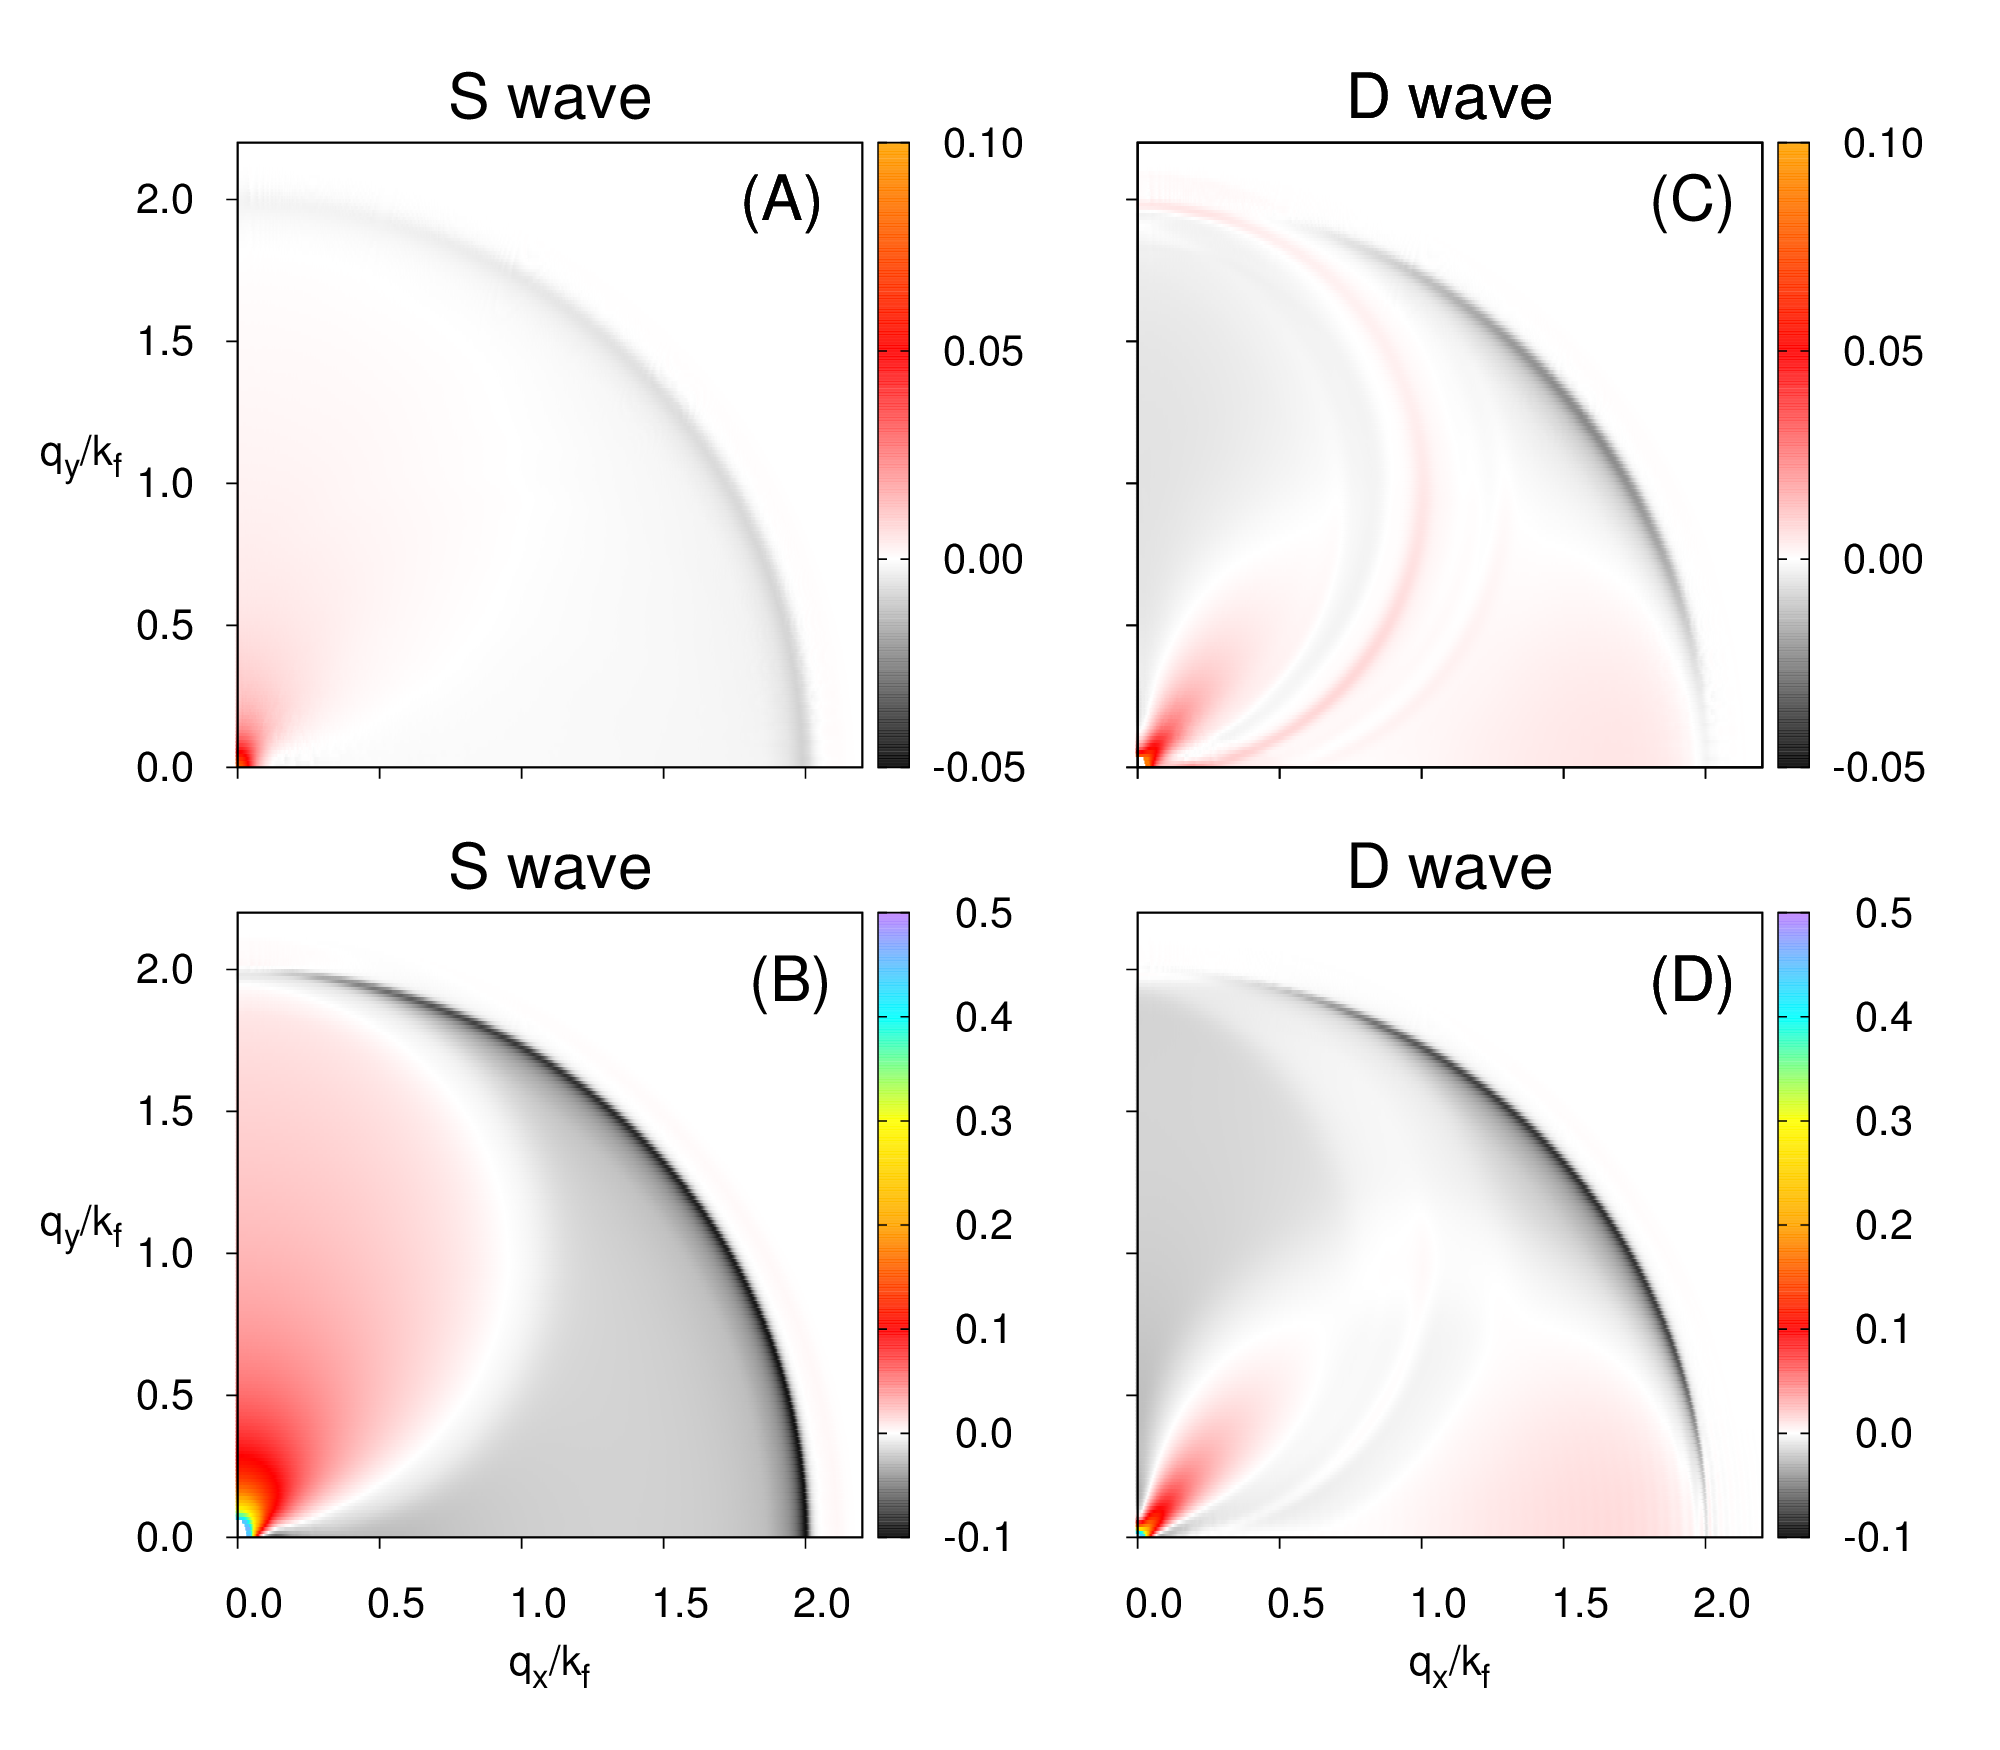
\includegraphics[scale=0.13]{./figures/fig2_SD_TB/Fig2_TB.png}
\caption{\label{fig:sus_TB}
Effects of magnetic field and temperature on  $\delta\chi'(\vq)$ at the center of domain wall. 
The zero-energy peaks are shifted by $\pm\mu_BH = \pm0.4\Delta_0$, significantly reducing 
AFM correlations. 
Panels are for different temperatures: 
(A) $k_B T = 0.35\Delta_0$;  
(C) $k_B T = 0.2\Delta_0$; 
(B,D) $k_B T = 0.05\Delta_0$. 
%Same temperature and field points are marked in figure \ref{fig:3_S} and \ref{fig:3_D}.  
\red{put (A,B,C,D) top left of each panel. Fix the color palette and contours.}
\blue{new figure attached. This is also $\delta\chi_{_I}$ not full $\delta\chi$. There is also a small spot of $\delta\chi>0.5$ near $q=0$ in (B) that is left white like fig \ref{fig:2}.}
} 
\end{figure}
%%%%%%%%%%%%%%%%%%%%%%%%%%%%%%%%%%%%%%%%%%%%%%%%%%%%%%%%%%%%%%%%%%%%%%%%%%%%%%%%

In external field the energies of spin-up/down quasiparticles are shifted by $\pm \mu_B H$, 
and the zero-energy peak is split into two peaks, separated by energy $2\mu_B H$. This leads to 
reduction of $\Pi^{\pm}$ factors (\ref{eq:fermi_factor}) 
and $\delta\chi$ shows very little enhancement over the normal state. 
In figure \ref{fig:sus_TB} we present $\delta\chi$ at the center of domain wall for applied field
$\mu_B H = 0.4\Delta_0$, close to Pauli field, $\mu_B H_P \approx 0.7 \Delta_0\; (S-wave),\; 0.55\Delta_0 (D-wave)$. 
At lower temperatures (panels B and D) the $H=0$ enhancement regions %that were present in $H=0$ 
are still distinguishable but are much smaller, including the $q=0$ uniform magnetization, since there is no 
zero-energy peak anymore. In $D$-wave the enhancement at antiferromagnetic $q_x \sim 1.75 k_f$ is 
almost entirely wiped out. 
The higher temperature plots in figure \ref{fig:sus_TB}A and \ref{fig:sus_TB}C
reveal a further reduction of $\chi'(\vq)$ due to a smaller self-consistent gap
and overall thermal smearing of the sum in (\ref{eq:sus}).   
We note that higher fields and temperatures mostly reduce correlation terms between bound states, 
while the coupling of bound states with the free states is largely unaffected. 
For these fields the free states will
actually be shifted closer to zero energy for the spin-up quasiparticles.
\red{These terms are responsible for slight enhancement at isotropic $|\vq| \gtrsim 2k_f$.}
\blue{these regions become suppressed also when using $2^{12}$ momentum points}
%
This suppression of $\delta\chi$ with magnetic field at the domain wall is manifestly opposite 
to behavior of susceptibility in the bulk, where magnetic field facilitates appearance of SDW 
correlations.\cite{sc_afm_kato,Rosemeyer2014} 
\red{Do you see it away from the DW?} \blue{yes, I can provide figure if you'd like}

%%%%%%%%%%%%%%%%%%%%%%%%%%%%%%%%%%%%%%%%%%%%%%%%%%%%%%%%%%%%%%%%%%%%%%%%%%%%%%%%
\begin{figure*}
\subfloat[$S$-wave \label{fig:3_S}]{
 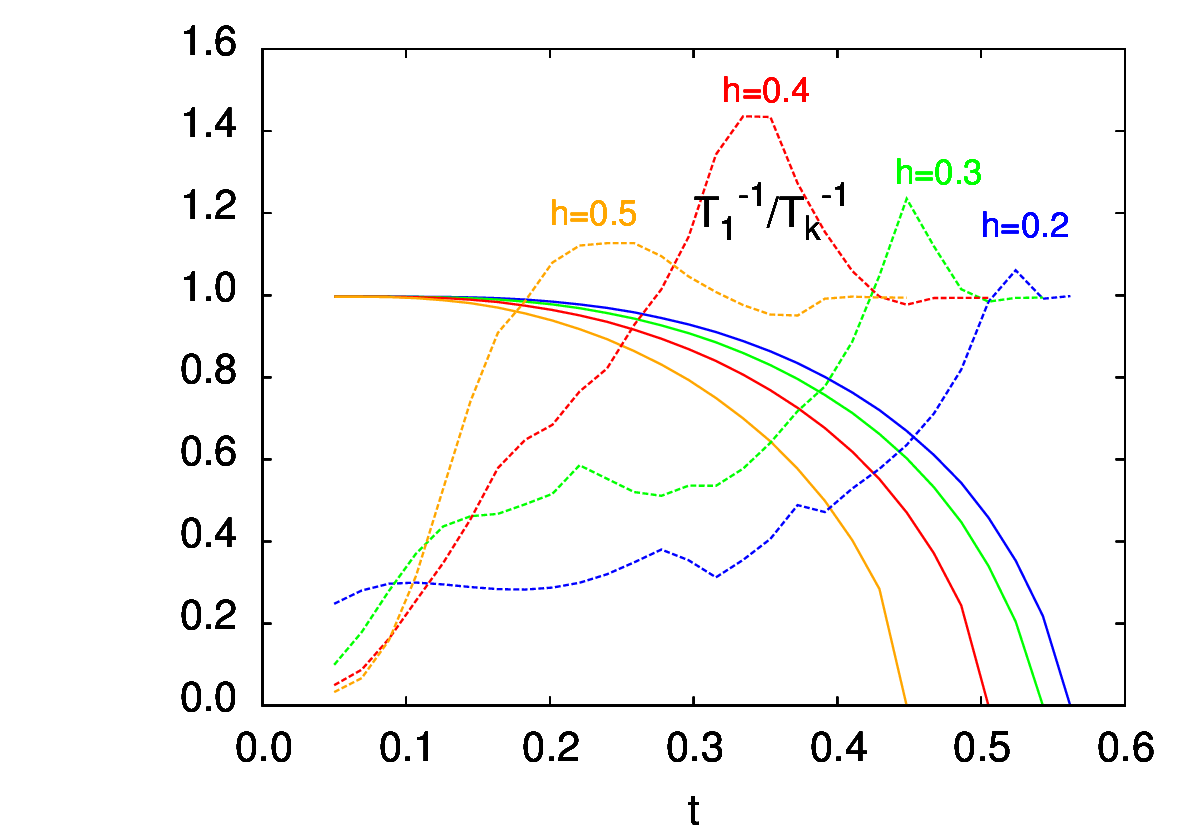
\includegraphics[scale=0.2]{./figures/fig_relTime_deltaTB/fig_relTime_deltaTB_S.png}
}
\hfill
\subfloat[$D$-wave \label{fig:3_D}]{
 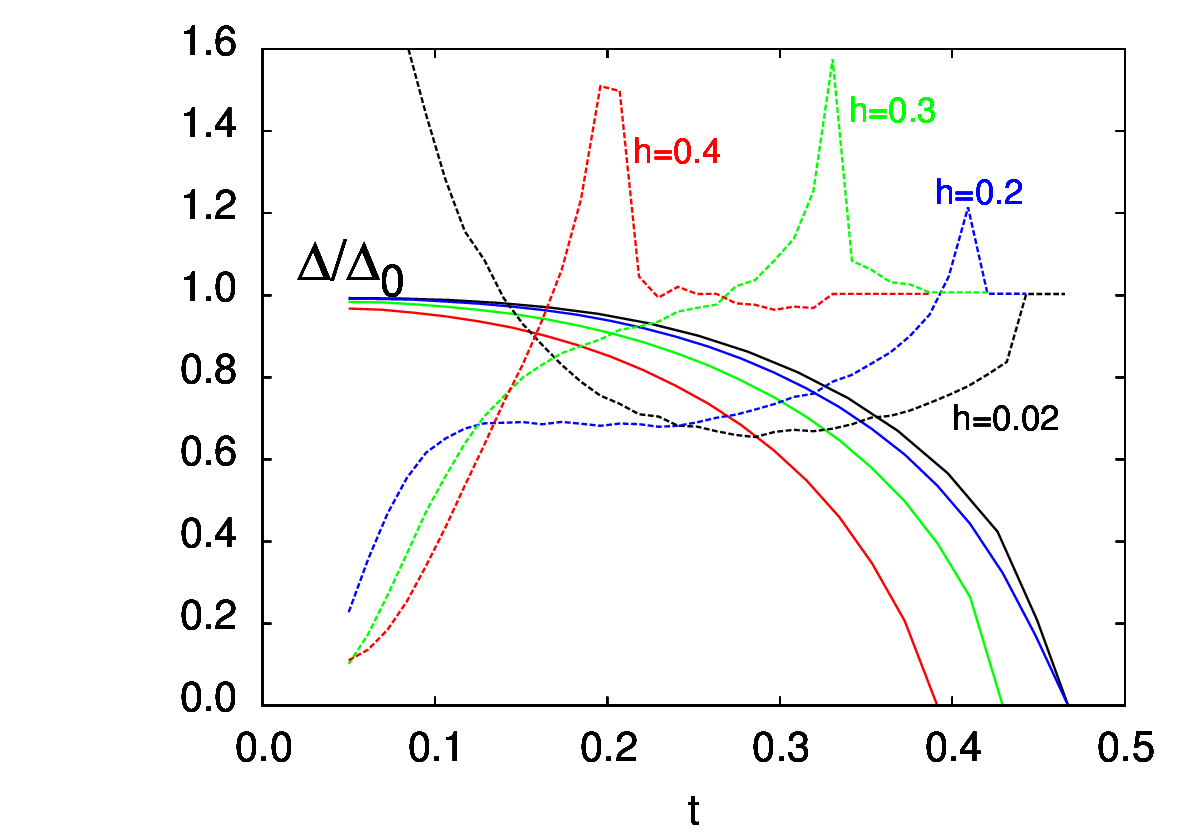
\includegraphics[scale=0.2]{./figures/fig_relTime_deltaTB/fig_relTime_deltaTB_D.png}
}
\caption{
The relaxation rate at the center of domain wall, 
normalized to the Korringa limit $T_1^{-1} / T_K^{-1}$ (dashed lines), 
and the bulk gap $\Delta/\Delta_0$ (solid lines) as a function of temperature $t = k_B T/\Delta_0$ 
for different applied fields $h = \mu_B H/\Delta_0$. 
The labelled points $A$, $B$, $C$, $D$ correspond to parameters used in figure \ref{fig:sus_TB} 
\red{- what is the importance of this relation between figures?} \blue{ (A) (B) (C) (D) label the T-H points taken for figure \ref{fig:sus_TB} I think I'll take them out in next version}. 
We set $\omega'=\omega'' = \Delta_0/100$ \red{-do you need it? Eq.~\ref{eq:T1} does not need $\omega'$ or $\omega''$}\blue{right. I will redo the plot using ~\ref{eq:T1} but I still have to use one parameter to numerically describe delta function. I will use a gaussian delta function for the numeric integration $e^{-(\epsilon_n-\epsilon_{n'})^2/10^{-6}}$}
The enhancement of the relaxation rate above normal state value is due to transitions between 
bound states and the continuum states, when $\Delta(T,H) = 2 \mu_B H$ (Fig. \ref{fig:rel_trans}).
\red{Too many duplicate statements. Remove legend. Put $\Delta/\Delta_0$ next to solid lines in one panel. 
Put $T_1^{-1} / T_K^{-1}$ next to dashed lines in another. Use better fonts. 
Why are lines so rugged? Use symbols and numerical error bars and a `guide to the eye' line if 
you cannot get rid of the noise. 
Why h=0.2 D-wave behavior looks so funny at low T? 
Can you put bulk $T^{-1}_1$ here for comparison? }\blue{I am working on a new figure, but having difficulty getting smooth...}
}
\end{figure*}
%%%%%%%%%%%%%%%%%%%%%%%%%%%%%%%%%%%%%%%%%%%%%%%%%%%%%%%%%%%%%%%%%%%%%%%%%%%%%%%%

%%%%%%%%%%%%%%%%%%%%%%%%%%%%%%%%%%%%%%%%%%%%%%%%%%%%%%%%%%%%%%%%%%%%%%%%%%%%%%%%
\begin{figure}
 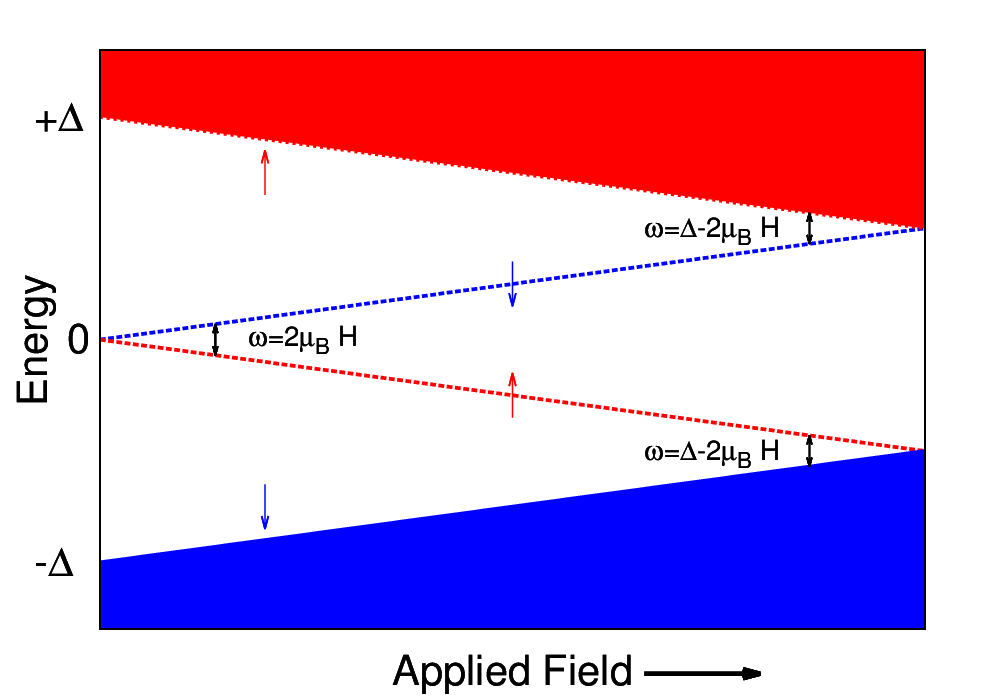
\includegraphics[scale=0.25]{./figures/fig_relTime_trans_2/Fig_rel_time_trans.png}
\caption{\label{fig:rel_trans}
Splitting of the energy states by Zeeman magnetic field. The bound states contribute to the relaxation rate 
$T_1^{-1}$ at the domain wall either at small fields, where transitions between spin-flipped bound states are allowed, 
or at fields $2\mu_B H = \Delta$ that allow transitions between bound states and the low-lying continuum 
states at $\Delta$. 
\red{Shade the continuum states above $+\Delta$, below $-\Delta$. Put spin arrows on actual lines, 
remove legend.}\blue{new figure attached}
}
\end{figure}
%%%%%%%%%%%%%%%%%%%%%%%%%%%%%%%%%%%%%%%%%%%%%%%%%%%%%%%%%%%%%%%%%%%%%%%%%%%%%%%%

%~~~~~~~~~~~~~~~~~~~~~~~~~~~~~~~~~~~~~
\subsection{Relaxation Rate}
\label{sec:T1}
%~~~~~~~~~~~~~~~~~~~~~~~~~~~~~~~~~~~~~
We also calculate the imaginary part of susceptibility 
taking $\omega''\rightarrow 0$ \blue{the last term is a minus! We can write $|A_{\vn\vn'}(\vx)|^2$ instead of $A_{\vn\vn'}(\vx)A^*_{\vn\vn'}(\vx)$}
\be
\begin{split}
\label{eq:sus_imag} \nonumber
&\chi_{_{\perp}}''(\vx,0,\omega') \propto \sum\limits_{\vn\vn'\mu} \\  %\int\,d\vr e^{-i\vq\cdot\vr} \\
&\left[   A_{\vn\vn'}(\vx)A^*_{\vn\vn'}(\vx) [f(\epsilon_{\vn\mu})-f(\epsilon_{\vn'\bmu})] 
		\delta(\omega'+\epsilon_{\vn\mu}-\epsilon_{\vn'\bmu}) \right. \\
    &    +C^*_{\vn\vn'}(\vx)C_{\vn\vn'}(\vx) [f(\epsilon_{\vn\mu})-f(-\epsilon_{\vn'\mu})] 
     		\delta(\omega'+\epsilon_{\vn\mu}+\epsilon_{\vn'\mu}) \\
& \left. +C_{\vn\vn'}(\vx)C^*_{\vn\vn'}(\vx) [f(\epsilon_{\vn\mu})-f(-\epsilon_{\vn'\mu})]
    		\delta(\omega'-\epsilon_{\vn\mu}-\epsilon_{\vn'\mu}) \right]
\end{split}
\ee
to find the local spin-lattice relaxation rate (\ref{eq:rel_time}) in static limit 
$T_1^{-1}(\vR,\omega') = A_0^2 2T [\chi''_{\perp}(\vR,\vr=0,\omega')/ \omega']_{\omega'\rightarrow 0}$: 
\be
\label{eq:T1}
\frac{1 }{T_1(\vx) T } =  
- 2 A_0^2 \sum\limits_{\vn\vn'\mu} \pder{f(\epsilon_{\vn\mu})}{\epsilon}
\left| A_{\vn\vn'}(\vx) \right|^2 \delta(\epsilon_{\vn\mu}-\epsilon_{\vn'\bmu}) \,.
\ee
\blue{the above should include a term with $|C|^2$ like this $\pder{f(\epsilon_{\vn\mu})}{\epsilon}
\left| C_{\vn\vn'}(\vx) \right|^2 \delta(\epsilon_{\vn\mu}+\epsilon_{\vn'\mu})$ coming from the minus sign in last term above. I will use this equation for $T_1^{-1}$ and for the delta function a Gaussian $e^{(\epsilon_{\vn}\pm\epsilon_{\vn'})^2/10^{-6}}$ }
%The high-energy part of this sum gives the trivial normal state result. 
%the contributions from the mixed low-high energy region $II$ are negligible in $\omega'\to 0$ static limit. 
%The reason for this are the $\delta$-functions that eliminate $CC^*$ terms (at least one of 
%$\epsilon > \Lambda$), and the $AA^*$ term vanishes because $\delta$-function argument 
%can be zero only if $\epsilon_{\vn\mu},\epsilon_{\vn'\mu'}$ are both near the cutoff, 
%$\Lambda \pm \mu_B H$, resulting in vanishing Fermi functions 
%$f(\epsilon_{\vn\mu})\approx f(\epsilon_{\vn'\mu'})\approx 0$. 

The deviations of relaxation rate from the normal state's Korringa limit\cite{Korringa1950601} 
are due to the spin-flip transitions between the low-energy states. 
Figures \ref{fig:3_S} and \ref{fig:3_D}
provide numeric results for relaxation rate at the domain wall for S- and D-wave symmetry, 
where the bulk order parameter $\Delta(T,H)$ is self-consistently determined for higher fields. 
In S-wave one notices that the usual coherence peak below $T_c$ for $H\to0$ is absent in the middle of the domain wall, 
due to spatial asymmetry of the order parameter. 
However, a peak develops for higher fields, but it lies not immediately below $T_c(H)$, but at lower temperatures. 
Similar enhancement of relaxation rate above the normal state's value can also be seen in D-wave. 
This peak appears due to transitions between the bound states and the continuum states, when 
$\epsilon_{\vk\mu} \sim \Delta \pm \mu_B H = \mp \mu_B H = \epsilon_{0\bmu}$ 
($\omega' \to 0$ limit), as schematically shown in figure \ref{fig:rel_trans}. 
Interestingly, the transitions between bound states can increase $T_1^{-1}$ beyond the
Korringa limit only for small fields $2\mu_B H \approx \omega' \to 0$. 
\red{Ans this can be seen WHERE in figures?} \blue{I will include a lower field curve in figure \ref{fig:3_S} and \ref{fig:3_D}}

% We end our analysis by noting that we have not presented results for higher
% fields above the Pauli limit $H_p$ because our self consistent method (see
% appendix) begins to break down for a single domain wall. This is not surprising
% because above $H_p$ is the FFLO regime where self consistent solutions require
% shorter wavelengths $\lambda_{fflo}$ which are on the order of $\xi_c$
% \cite{Vorontsov2005fflo}. Although we can initialize our self consistency to
% include this effect and achieve self consistent solutions, the goal of this
% report is to gain insight into the magnetic response near a $\emph{single}$
% domain wall, and we leave further investigation into bound state hybridization
% effects and inter-DW coupling for future works.

%~~~~~~~~~~~~~~~~~~~~~~~~~~~~~~~~~~~~~
\section{Conclusions and discussion}
\label{sec:concl}
%~~~~~~~~~~~~~~~~~~~~~~~~~~~~~~~~~~~~~
%

To summarize, we found that the concentration of zero-energy Andreev bound states at a domain wall 
defect in the order parameter leads to significant enhancement of the bare 
susceptibility. Since variations of the order parameter occur on scale of coherence length $\xi_c \gg 1/k_f$, 
the new quasiparticle environment inside the domain wall may lead to overall divergence of the total 
\emph{local} susceptibility
$$
\chi^{RPA}(\vq,\vR) = \frac{ \chi_\perp(\vq,\vR)}{1 - J_\vq \, \chi_\perp(\vq,\vR) }
$$
for antiferromagnetic ordering vector $\vq$ ($q \sim k_f$), given sufficiently 
large exchange interaction $J_\vq$. This supports previous results of interplay between FFLO-type  
superconducting order parameter and the antiferromagnetic order in lattice models.\cite{Yanase2009abs,Marcin2009}
However, our weak-coupling approach with a single domain wall leads to results that differ 
considerably from the lattice models which used $q_{FFLO} \sim 1/\xi_c \sim q \sim k_f$. 

We find that the direction of the SDW modulation vector depends on the symmetry of 
the order parameter and the relative orientation of the domain wall and the nodes. 
For $S$-wave gap, $\vq$ is along the domain wall (i.e. $\vq \perp \vq_{FFLO}$), 
while for $D$-wave with nodes along the DW $\vq$-vector points across the domain wall. 
The susceptibility enhancement is related to the increased correlations between 
bound states. 
These correlations disappear with magnetic field and temperature, something that was not seen in lattice models. 
\red{Other?!}\blue{We can take this sentence out} regions of increased
susceptibility are more robust to changes in temperature and field and are due
to correlations between bound and propagating states. 

Applying our results to the \cecoin\ discussion, we can say that the scenario of FFLO-induced magnetism 
does not hold. First, the Q-phase appears in high magnetic fields\cite{cecoin5_Kenzelmann, cecoin5_Kenzelmann2} 
where we find bound state enhancement effects are wiped out. 
This high-field phase is rather more in line with susceptibility behavior in uniform state.\cite{sc_afm_kato,Rosemeyer2014} 
Moreover, even if the enhancement of susceptibility survives the field, 
from our calculation the direction of the SDW modulation is expected to be along the field 
(assuming $\vq_{FFLO} || nodes || H$) inconsistent with observations.\cite{Gerber2014}

On the other hand, we find increase of the spin-lattice relaxation rate $T_1^{-1}$ 
over the normal Korringa limit in high fields. This enhancement mostly appears due to transitions 
between bound states and the free propagating continuum states that can occur in high fields. 
This result is
qualitatively similar to that seen in \kbtf\ near the superconducting-normal transition,\cite{Mayaffre2014} 
indicating presence of low-energy states inside the superconducting gap associated with 
non-uniform superconducting phase. 

%We end by noting that our method of solving the BdG equations is a novel
%approach which allows for finite wave vector calculations of observables while
%only keeping the low energy excitations near $k_f$.

\section{Acknowledgements}

We thank Caroline Richard for helpful discussions and 
acknowledge support from NSF through grant DMR-0954342. 



%%%%%%%%%%%%%%%%%%%%%%%%%%%%%%%%%%%%%%%%%%%%%%%%%%%%%%%%%%%%%%%%%%%%%%%%%%%%%
%%%%%%%%%%%%%%%%%%%%%%%%%%%%%%%%%%%%%%%%%%%%%%%%%%%%%%%%%%%%%%%%%%%%%%%%%%%%%
\appendix*

\section{Self-consistent order parameter}
\label{app:self-cons}

To calculate susceptibility $\chi(\vq,\vR)$, which is a function
of relative momentum $\vq$, we choose a natural momentum-based Fourier
expansion (\ref{eq:wave_exp}) to find 
self-consistent solutions of BdG amplitudes $u_\vn(\vx),v_\vn(\vx)$ from (\ref{eq:BdG}) with order parameter
(\ref{eq:delta}). 
In the past, a variety of numeric or approximate
methods have been used to address this problem: 
\cite{PhysRevLett.105.167006, Vorontsov2005fflo, PhysRevLett.80.4763, RevModPhys.76.263, RevModPhys.77.935,
JPSJ.68.3120, PhysRevB.57.8709, PhysRevLett.110.131601} 
spatial lattice,\cite{appropriate}
Chebyshev polynomial expansion\cite{appropriate} or
quasiclassical Greens functions.\cite{appropriate} 
Though effective, they are less suitable for our purpose. 

The separable order parameter $\Delta(\vx,\vx')=\Delta(\vR) g(\vr)$ 
with relative $\vr=\vx-\vx'$ and center-of-mass $\vR=(\vx+\vx')/2$ coordinates 
is obtained from mean-field definition (\ref{eq:delta}) using Bogoliubov transformation (\ref{eq:BdG_trans}):
\begin{align}
\begin{split}
\Delta(\vR) \, g(\vr) = V(\vr) \sum\limits_{\vn}{}^{'}\left\{ 
u_{\vn}(\vx) v^*_{\vn}(\vx') \left[ f(\epsilon_{\vn\downarrow}) + f(\epsilon_{\vn\uparrow}) \right] \right.
\\
\left.
- u_{\vn}(\vx') v^*_{\vn}(\vx) \left[ f(-\epsilon_{\vn\downarrow}) + f(-\epsilon_{\vn\uparrow}) \right]
\right\}
\end{split}
\label{eq:selfcon0}
\end{align}
where $f(\epsilon_{\vn\mu}) = \langle \gamma^\dagger_{\vn\mu}\gamma_{\vn\mu}
\rangle$ is the Fermi occupation number of state $\epsilon_{\vn\mu}$ with spin $\mu$. 
The prime on the sum denotes the cut-off restriction on the attractive potential $V(\vr)$, 
$|\epsilon_{\vn}|<\Lambda$,\cite{PhysRevLett.80.4763} 
which for this report we set at $\Lambda = 5\Delta_0$, 
where $\Delta_0 = 0.05\epsilon_f$ is the zero temperature bulk order parameter. 
The amplitude of the order parameter is decomposed into CoM momentum $Q$ (only $x$-component for the domain wall) 
\be
\Delta(R_x) = \int dQ \;  \tilde{\Delta}(Q) \, e^{iQR_x} \,.
\ee
Using the Fourier expanded amplitudes (\ref{eq:wave_exp}) for momenta $p$ along the domain wall, 
and $k=\{k_i\}$ in $x$ direction, and introducing relative momentum, 
$\vr \to \vq$, we write the gap equation 
\begin{align}
\begin{split}
\tilde{\Delta}(Q)\, g_{\hq} = \sum\limits_{\vn,p, k}{}^{'} \tilde{u}_{\vn}(k) \tilde{v}^*_{\vn}(k-Q) 
\qquad\qquad\qquad
\\  
\bigg\{ \tilde{V}(\vq-\vK) \left[f(\epsilon_{\vn\downarrow}) + f(\epsilon_{\vn\uparrow})\right] 
\qquad
\\
-\tilde{V}(\vq+\vK)\left[f(-\epsilon_{\vn\downarrow}) + f(-\epsilon_{\vn\uparrow})\right] \bigg\}
\end{split}
\label{eq:selfcon1}
\end{align}
Here $\vK = (k-Q/2)\hx + p\hy$, with magnitude $|\vK|,|\vq|\sim k_f$. We take separable 
interaction $\tilde{V}(\vq-\vK) = - V \, g_{\hat{q}} \, g^*_{\hat{K}}$ with a constant $V$. 
Then 
\be
\tilde{\Delta}(Q) = V \sum\limits_{\vn,p, k, \mu}{}^{'} 
\tilde{u}_{\vn}(k) \tilde{v}^*_{\vn}(k-Q)g_{\hat{K}} \tanh \left[\frac{\epsilon_{\vn\mu}}{2T}\right] 
\label{eq:selfcon2}
\ee
The interaction parameter $V$ is eliminated together with the cut-off $\Lambda$ 
using the zero temperature and field value $\Delta_0$. 
We recursively solve (\ref{eq:BdG_mat}) with 
(\ref{eq:selfcon2}) until sufficient convergence for profile  $\Delta(R_x)$ is reached. 

%%%%%%%%%%%%%%%%%%%%%%%%%%%%%%%%%%%%%%%%%%%%%%%%%%%%%%%%%%%%%%%%%%%%%%%%%%%%%
%%%%%%%%%%%%%%%%%%%%%%%%%%%%%%%%%%%%%%%%%%%%%%%%%%%%%%%%%%%%%%%%%%%%%%%%%%%%%
%~~~~~~~~~~~~~~~~~~~~~~~~~~~~~~~~~~~~~~~~~~~~~~~~~~~~~~~~~~~~~~~~~~~~~~~~~~~~~~~%
\bibliography{./mybib}
\end{document}
%~~~~~~~~~~~~~~~~~~~~~~~~~~~~~~~~~~~~~~~~~~~~~~~~~~~~~~~~~~~~~~~~~~~~~~~~~~~~~~~%

